%!TEX program = xelatex
\documentclass[12pt,a4paper]{article}
\usepackage{graphicx}
\usepackage{geometry}
\usepackage{booktabs}
\usepackage{cite}
\usepackage{amsmath,amssymb}
\usepackage{hyperref}
\usepackage{multirow}
\usepackage{array}
\usepackage{xcolor}
\usepackage{colortbl}
\usepackage{longtable}
\usepackage{pdflscape}
\usepackage{caption}
\usepackage{subcaption}
\usepackage{float}
\usepackage{url}
\usepackage{enumitem}
\usepackage{microtype}
\geometry{a4paper, margin=1in}
\captionsetup{font=small, labelfont=bf, skip=6pt}
\usepackage{iftex}
\ifXeTeX
  \usepackage{fontspec}
  \newfontfamily\banglafont[Script=Bengali]{Kalpurush}
\else
  \providecommand{\banglafont}{}
\fi
\ifdefined\DeclareUnicodeCharacter
  \DeclareUnicodeCharacter{0964}{\textbar}
\fi

\begin{document}

\begin{titlepage}
    \centering
    
    \vspace*{1cm}
    
    \Large
    \textbf{B.Sc in Computer Science and Engineering Thesis Report on}
    
    \vspace{1.5cm}
    
    \Huge
    \textbf{Poly-Dialectal Neural Machine Translation System for Bangla Regional Dialects}
    
    \vspace{2cm}
    
    \Large
    \textbf{Submitted By}\\
    \vspace{0.5cm}
    \large
    \textbf{Rakib Ullah} \\
    Reg No: 2020331520 \\
    \vspace{0.3cm}
    \textbf{Ruhul Islam Rahul} \\
    Reg No: 2020331529 \\
    \vspace{0.3cm}
    \textbf{Tanbir Ahmed} \\
    Reg No: 2020331516 \\
    
    \vspace{2cm}
    
    \Large
    \textbf{Supervised By}\\
    \vspace{0.5cm}
    \large
    \textbf{Nayan Kumar Nath} \\
    Lecturer \\
    Department of Computer Science and Engineering, \\
    Sylhet Engineering College \\
    
    \vfill
    
    \Large
    \textbf{Department of Computer Science and Engineering}\\
    \vspace{0.2cm}
    \LARGE
    \textbf{SYLHET ENGINEERING COLLEGE, SYLHET}\\
    \vspace{0.5cm}
    \large
    Affiliated with\\
    \Large
    \textbf{Shahjalal University of Science and Technology}\\
    \large
    Sylhet, Bangladesh.\\
    \vspace{0.8cm}
    \large
    22 August, 2026
    
\end{titlepage}

\newpage

\begin{abstract}
\noindent
Bangla, an Indo-Aryan language spoken by over 240 million people, encompasses substantial regional dialectal diversity spanning variants such as Sylheti, Chittagonian, Barisali, Noakhali, and Mymensingh. These dialects diverge markedly from Standard Colloquial Bangla (SCB) in phonology, morphology, syntax, and lexicon, creating significant communication barriers and systemic exclusion from digital language technologies. Existing neural machine translation (NMT) systems and large language models (LLMs) treat Bangla as a monolithic entity, lacking the capacity to handle intra-language dialectal variation. This thesis introduces a unified poly-dialectal NMT framework that enables multi-directional translation across three paradigms: Dialect$\rightarrow$Standard Bangla, Standard Bangla$\rightarrow$Dialect, and direct Dialect$\rightarrow$Dialect---eliminating cascading errors inherent in pivot-based approaches. We construct the largest multi-dialectal parallel corpus for Bangla to date, comprising 51,531 non-null parallel sentence pairs across 11 regional variants by integrating seven existing datasets and 2,500 manually created, expert-verified sentence pairs for five previously unaddressed dialects. A systematic benchmarking of three NMT architectures---BanglaT5 (247M), NLLB-200 (615M), and mBART-50 (611M)---under parameter-efficient Low-Rank Adaptation (LoRA) fine-tuning reveals that language-specific pre-training substantially outperforms massively multilingual models. Extended 100-epoch training of BanglaT5 achieves a BLEU score of 29.26 and chrF++ of 57.26, surpassing the previous state-of-the-art by 5.59 BLEU points. A controlled dataset scaling study demonstrates that translation quality improves by 113\% as data scales from 500 to 4,499 parallel pairs, with diminishing returns beyond 3,000 samples. The system is deployed as a publicly accessible, INT8-quantized web application providing real-time translation services.

\vspace{0.5cm}
\noindent
\textbf{Keywords:} Neural machine translation, Bangla regional dialects, poly-dialectal translation, low-resource NLP, parameter-efficient fine-tuning, LoRA, BanglaT5, digital inclusion
\end{abstract}

\newpage

\section{Introduction}

\subsection{Background and Motivation}
Bangla (Bengali), an Indo-Aryan language, is one of the most widely spoken languages globally, with over 240 million native speakers distributed primarily across Bangladesh and the Indian states of West Bengal, Tripura, and Assam. Despite its socio-linguistic prominence and rich literary heritage, Bangla is not a monolithic entity; rather, it exhibits substantial intra-language diversity through numerous distinct regional dialects. Variants such as Sylheti, Chittagonian, Barisali, Noakhali, Rangpuri, Rajshahi, and Mymensingh diverge from Standard Colloquial Bangla (SCB) across multiple linguistic strata, manifesting as profound phonological variations, complex morphological inflections, altered syntactic structures, and highly localized lexical choices. In the case of Chittagonian and Sylheti dialects, the degree of linguistic deviation is sufficiently severe that mutual intelligibility with Standard Bangla is substantially impaired \cite{faria2025vashantor}.

This intra-language divergence engenders significant communication barriers within the broader socio-economic framework. Native speakers of peripheral regional dialects frequently encounter difficulties in formal interactions, legal proceedings, and educational contexts traditionally conducted in Standard Bangla. Furthermore, modern Natural Language Processing (NLP) tools, machine translation systems, and digital interfaces---ranging from virtual assistants to automated governance platforms---are overwhelmingly optimized exclusively for Standard Bangla. Consequently, millions of dialectal speakers face systemic digital marginalization and language-access inequality, lacking automated communication technologies adapted to their native spoken forms. This technological disparity underscores an urgent need for inclusive NLP systems capable of bridging the communication gap without enforcing linguistic homogenization.

\subsection{Problem Statement}
In recent years, Neural Machine Translation (NMT) architectures and Large Language Models (LLMs) have achieved state-of-the-art results for cross-lingual tasks involving high-resource languages. However, their efficacy degrades substantially when applied to low-resource intra-language dialectal shifts. Most existing Bangla NLP benchmarks and pre-trained models treat the language as a singular, uniform distribution, fundamentally disregarding the complex cross-dialectal matrix.

This limitation stems from a confluence of critical technical challenges. First, there is an acute scarcity of multi-dialectal parallel corpora required to effectively fine-tune deep neural networks. Second, the lack of standardized orthography for regional dialects exacerbates tokenization mismatches; standard Byte-Pair Encoding (BPE) \cite{sennrich2015neural} or WordPiece \cite{wu2016google} algorithms optimized for SCB frequently fragment dialectal words into semantically incoherent subwords. Third, existing regional text datasets suffer from severe class imbalance and are predominantly designed for classification tasks rather than complex generative alignment.

Formally, the poly-dialectal translation problem can be defined as follows. Let $\mathcal{D} = \{d_1, d_2, \ldots, d_k\}$ denote the set of $k$ regional dialect variants (including SCB). Given a source sentence $\mathbf{x} = (x_1, x_2, \ldots, x_m)$ in dialect $d_s \in \mathcal{D}$ and a target dialect $d_t \in \mathcal{D}$ where $d_s \neq d_t$, the objective is to learn a unified translation function $\mathcal{T}_\theta: (\mathbf{x}, d_s, d_t) \rightarrow \mathbf{y}$ that generates the target sentence $\mathbf{y} = (y_1, y_2, \ldots, y_n)$ such that $\mathbf{y}$ is a semantically faithful and morphologically authentic rendering of $\mathbf{x}$ in $d_t$. Addressing this challenge requires a paradigm shift from uni-dialectal modeling to a holistic, poly-dialectal approach.

\begin{figure}[htbp]
  \centering
  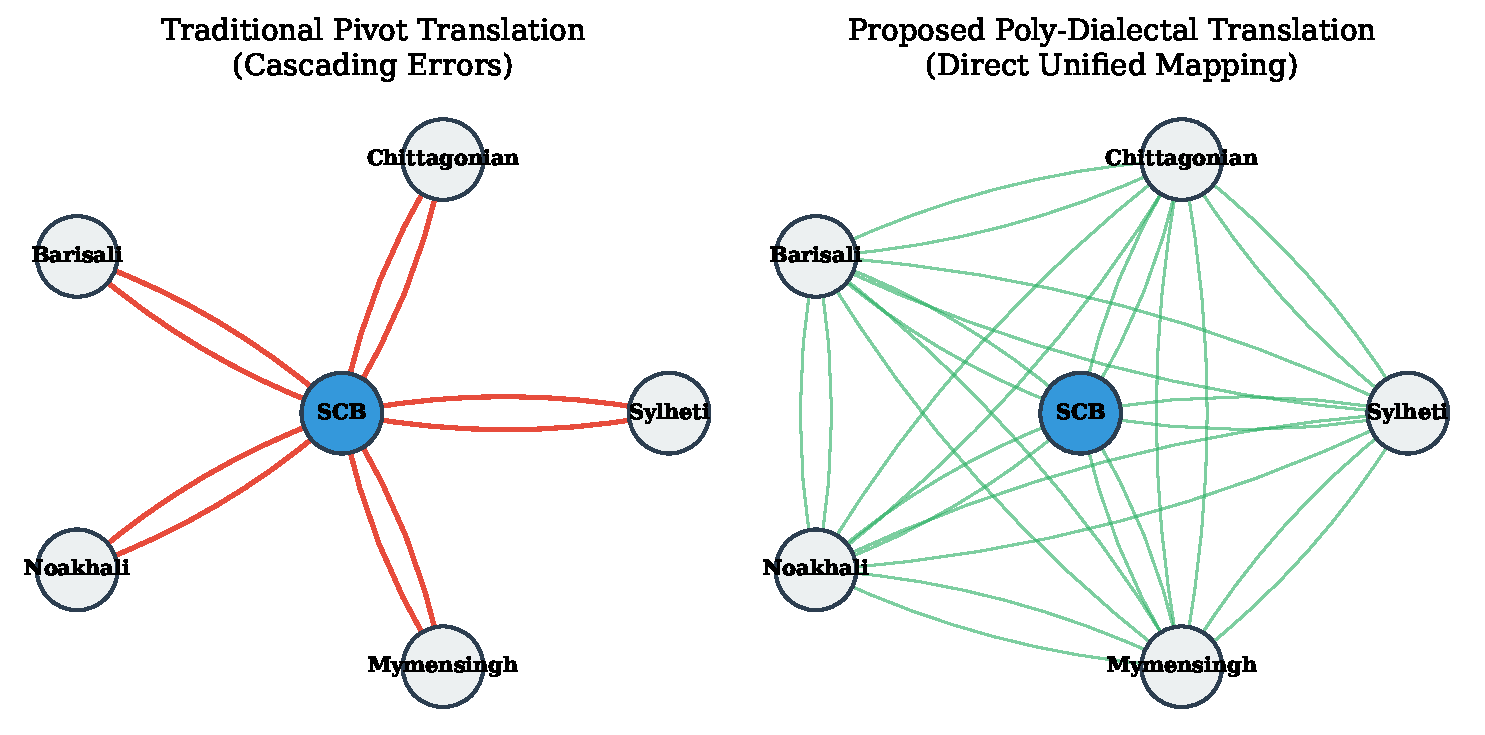
\includegraphics[width=\textwidth]{graphics/topology_comparison.pdf}
  \caption{Structural comparison between the traditional pivot translation approach (routing through Standard Bangla) and the proposed direct poly-dialectal mapping topology.}
  \label{fig:topology}
\end{figure}


\subsection{Proposed System and Contributions}
To address these limitations, this research introduces a unified \textbf{Poly-Dialectal Neural Machine Translation System} tailored for the morphological and syntactic nuances of Bangla regional dialects. As illustrated in Figure~\ref{fig:overview}, our architecture enables multi-directional translation across three core operational paradigms: Dialect $\rightarrow$ Standard Bangla, Standard Bangla $\rightarrow$ Dialect, and direct Dialect $\rightarrow$ Dialect translation, thereby eliminating the cascading errors typically introduced by pivot-based translation methods.

\begin{figure}[htbp]
  \centering
  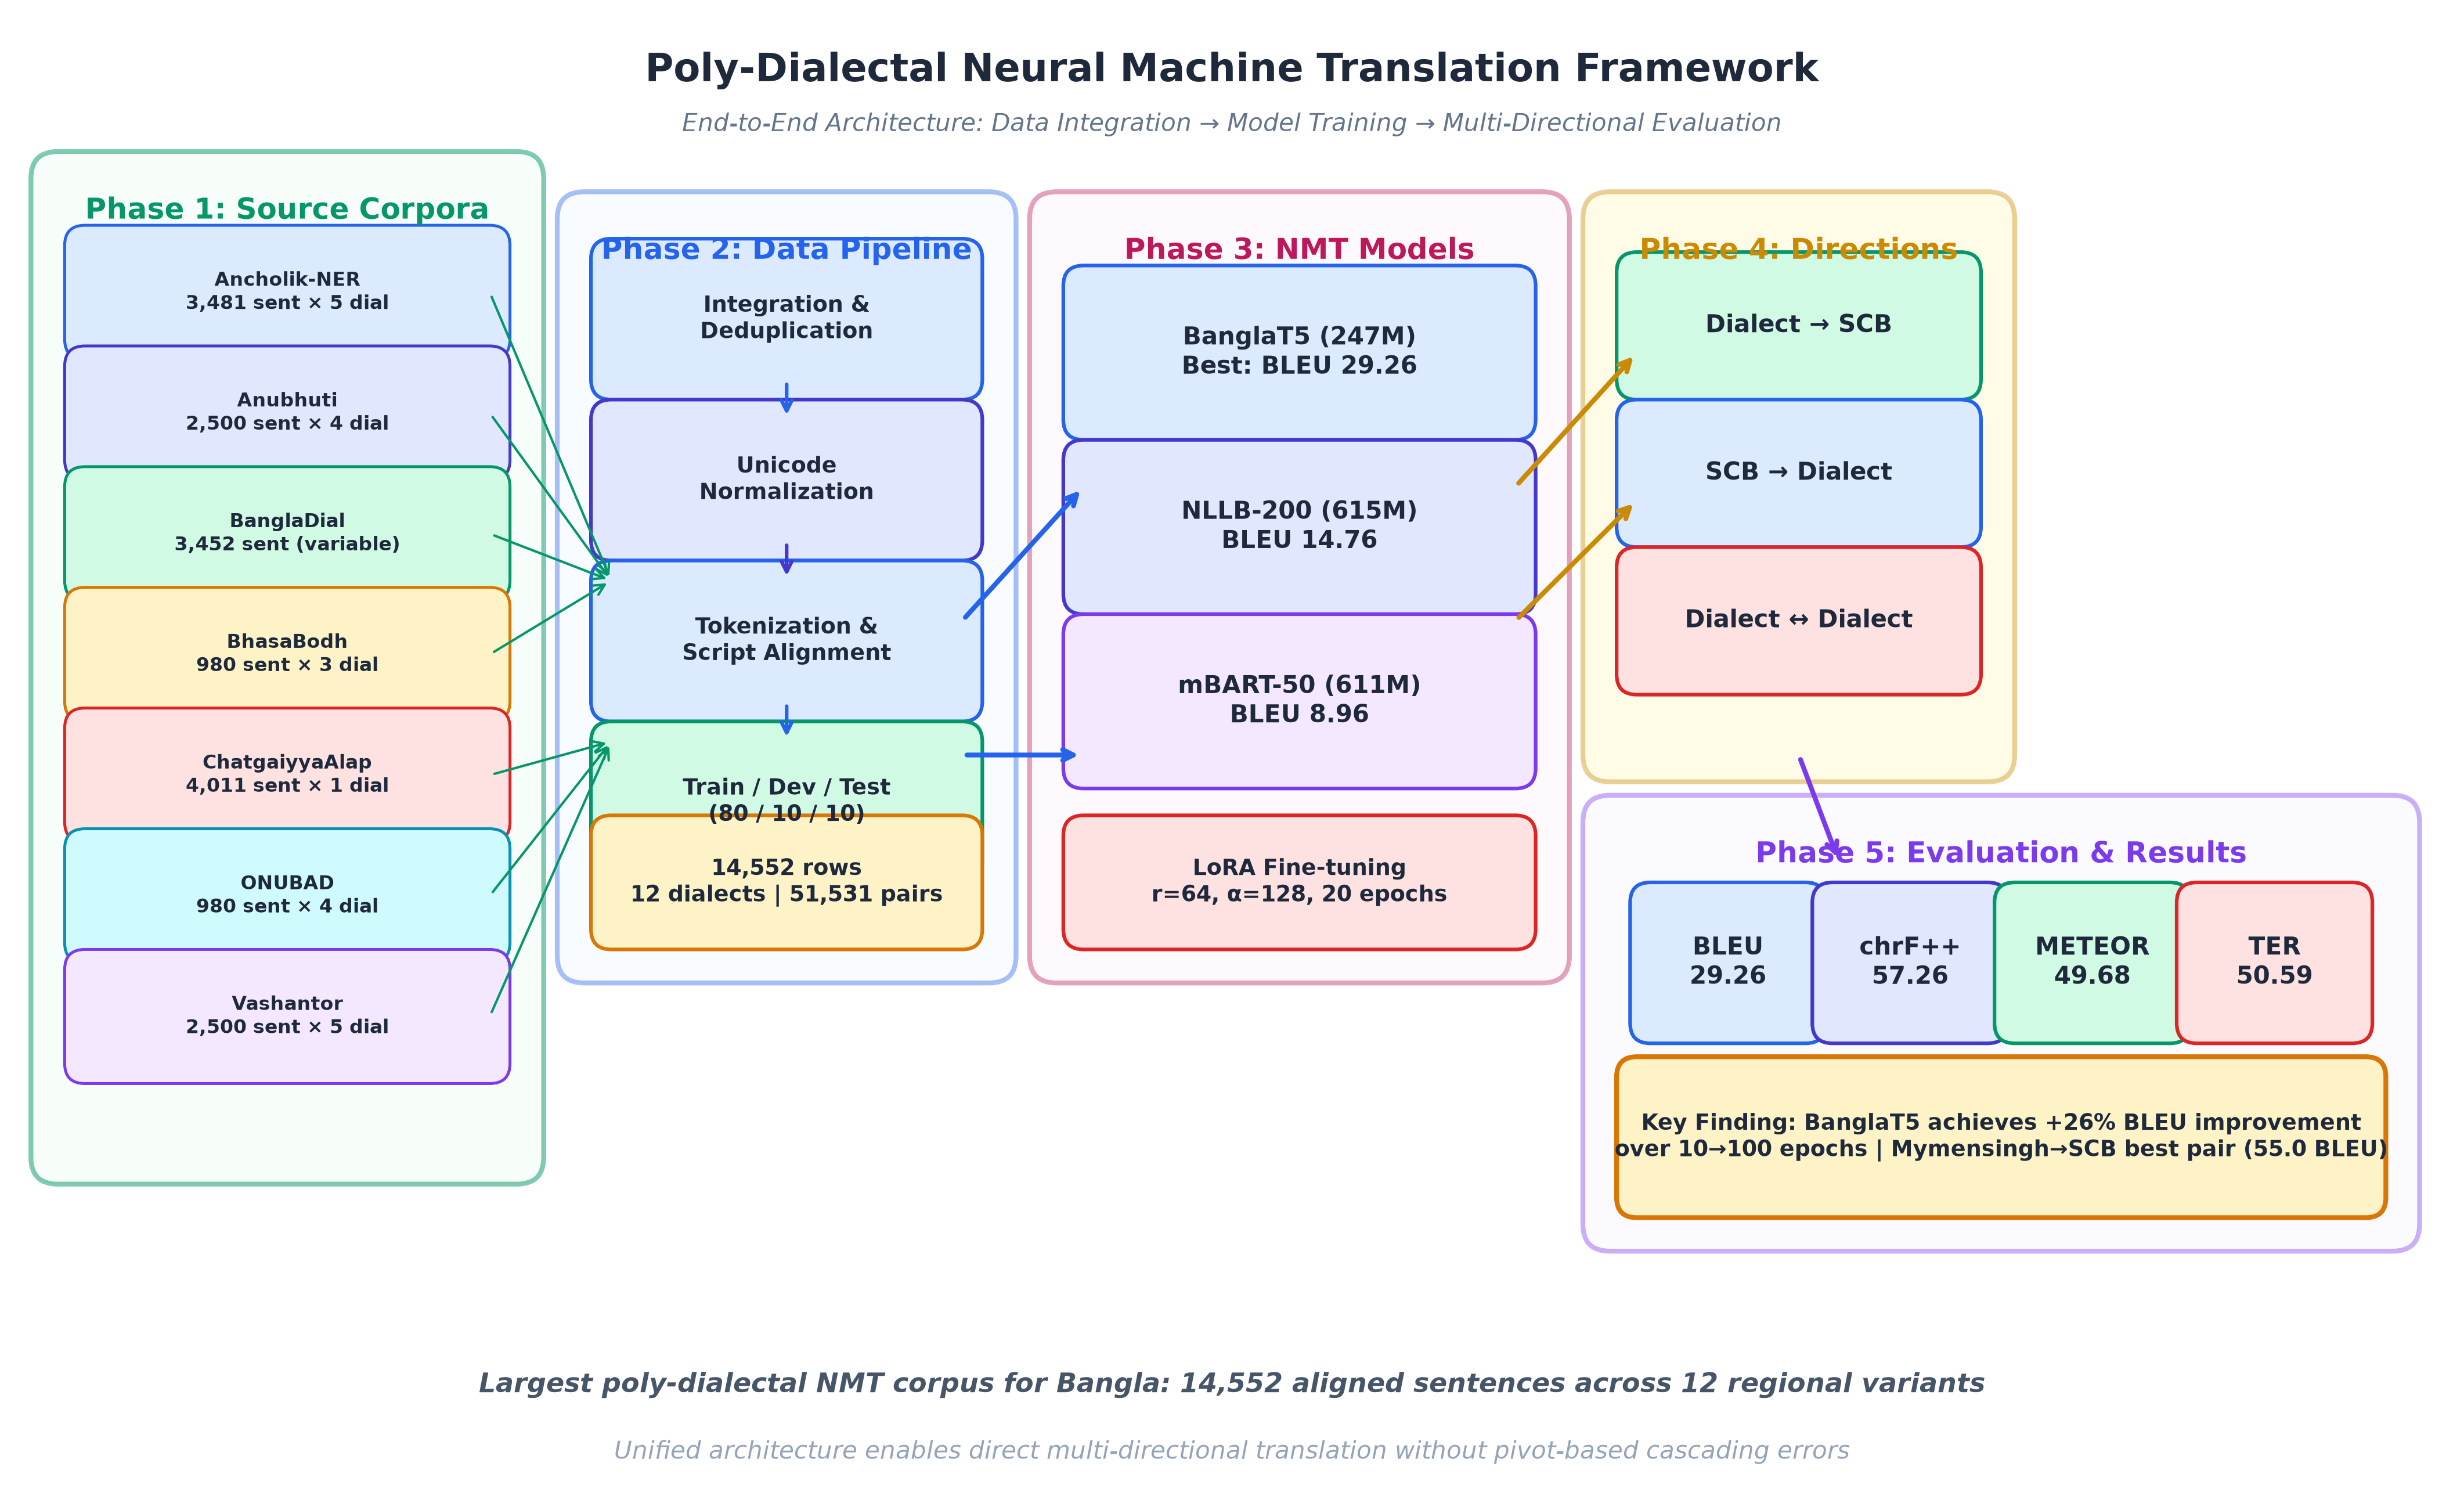
\includegraphics[width=0.95\textwidth]{graphics/overview.png}
  \caption{End-to-end architectural workflow of the Poly-Dialectal Neural Machine Translation Framework, depicting five phases: source corpora integration from seven existing datasets, the data processing pipeline, NMT model fine-tuning with LoRA, multi-directional translation paradigm, and evaluation with four standard MT metrics.}
  \label{fig:overview}
\end{figure}

The primary contributions of this thesis are summarized as follows:
\begin{enumerate}[leftmargin=*]
    \item \textbf{Largest Multi-Dialectal Parallel Corpus:} We construct the most extensive multi-dialect machine translation corpus for Bangla to date, comprising 14,552 aligned rows across 12 regional dialect columns. The corpus integrates seven prior datasets---Ancholik-NER, Anubhuti, BanglaDial, BhasaBodh, ChatgaiyyaAlap, ONUBAD, and Vashantor---and incorporates 2,500 manually created, bidirectional, expert-verified parallel sentence pairs for five previously unaddressed dialects (Rangpur, Tangail, Kishoreganj, Narail, Narsingdi), yielding 51,531 non-null parallel pairs across 11 regional variants.
    \item \textbf{Systematic Benchmarking of NMT Architectures for Poly-Dialectal Translation:} To the best of our knowledge, this work presents the first systematic empirical evaluation of prominent sequence-to-sequence architectures---specifically BanglaT5 \cite{bhattacharjee-etal-2023-banglanlg}, NLLB-200 \cite{nllb2022}, and mBART-50 \cite{tang2020multilingual}---on the task of multi-directional, poly-dialectal Bangla translation under parameter-efficient fine-tuning.
    \item \textbf{Cross-Dialectal Transfer Analysis and Dataset Scaling Study:} We conduct a rigorous dataset scaling study (progressively scaling from 500 to 4,499 parallel instances) and quantitative characterization of cross-dialectal transfer mechanisms, revealing how morphological proximity and training data volume jointly influence translation efficacy across diverse evaluation metrics.
    \item \textbf{Real-World Web Deployment:} We deploy the best-performing NMT model as a publicly accessible, INT8-quantized web application, enabling real-time poly-dialectal translation across 11 dialects and bridging the digital language divide for marginalized dialect speakers.
\end{enumerate}

\subsection{Thesis Organization}
The remainder of this report is organized as follows. Section~2 critically reviews related literature on Bangla regional NLP and dialectal machine translation. Section~3 formally states the research hypothesis and objectives. Section~4 details the methodology, encompassing dataset construction, model architectures, and fine-tuning configurations. Section~5 presents the experimental results, including cross-dialectal analysis, error taxonomy, dataset scaling findings, and comparison with prior art. Section~6 describes the deployment architecture and the publicly available web application. Section~7 discusses limitations and proposes future research directions. Section~8 concludes the thesis.

\newpage


\section{Literature Review}

\subsection{Overview of Regional Bangla NLP}
The development of linguistic resources for Bangla has historically favored Standard Colloquial Bangla, leaving regional dialects severely underrepresented in the NLP ecosystem. However, interest in low-resource regional Bangla NLP has grown substantially in recent years, with initial studies focusing on resource creation for text classification and sentiment analysis.

Sultana et al.~\cite{sultana2024bdregion} established the \textit{BdRegionText} corpus for regional text classification, demonstrating that standard classifiers exhibit significant performance degradation when exposed to dialectal vocabulary. Their best model (Random Forest with TF-IDF) achieved 79.15\% accuracy, revealing the representational gap between standard and regional text distributions. Building on this foundation, Mahi et al.~\cite{mahi2025bangladial} released \textit{BanglaDial}, a merged dataset spanning 11 dialects and Standard Bangla with 60,729 sentences, which quantified the severe class imbalance pervading available dialectal data (Imbalance Ratio $IR = 9.82$; Shannon Entropy $H = 3.416$ bits).

In specialized downstream tasks, the complexity of dialectal morphology presents additional challenges. Kundu et al.~\cite{kundu2026anubhuti} introduced \textit{ANUBHUTI}, targeting sentiment analysis across four regional variants with high inter-rater agreement (Cohen's $\kappa = 0.76$--$0.84$), revealing that emotion markers vary significantly across regional boundaries. Fayaz et al.~\cite{fayaz2025bidwesh} developed \textit{BIDWESH} for hate speech detection, demonstrating that SCB-trained toxicity classifiers fail to generalize to dialectal slang---a finding with direct implications for content moderation at scale. Paul et al.~\cite{paul2025ancholik} contributed \textit{ANCHOLIK-NER}, providing the first dialectal named entity annotations across Sylheti, Chittagonian, and Barisali variants. Notably, all three studies share a common limitation: they address classification tasks and do not provide generative capabilities for cross-dialectal communication.

\subsection{Dialectal Machine Translation and LLM Benchmarks}
Direct efforts in generative machine translation for Bangla dialects have emerged only recently, driven by the advent of massively multilingual neural models. Early translation corpora were highly localized: Chowdhury et al.~\cite{chowdhury2025chatgaiyya} constructed \textit{ChatgaiyyaAlap}, a parallel corpus of 4,012 sentences strictly for Chittagonian-to-Standard Bangla conversion. While valuable for the Chittagonian community, this resource inherently cannot support multi-directional or cross-dialectal translation. Sultana et al.~\cite{sultana2025onubad} presented \textit{ONUBAD} with 7,950 parallel rows spanning three dialects, establishing initial NMT baselines with BanglaT5 and SeamlessM4T. Faria et al.~\cite{faria2025vashantor} introduced \textit{Vashantor}, a multilingual benchmark covering five dialects with custom DialectBanglaT5 and DialectBanglaBERT models, achieving 71.93 BLEU on Mymensingh translation. However, \textit{Vashantor} was constrained to 2,500 sentences per dialect---a volume insufficient for robust generalization across diverse linguistic phenomena.

More recently, the research community has explored the capabilities of Large Language Models (LLMs) for dialect translation. Mahjabin et al.~\cite{mahjabin2025banglachq} constructed \textit{BanglaCHQ-Prantik} to benchmark LLMs in the medical domain, where Gemini 2.5 Flash achieved 23.67 BLEU on Sylheti translation. Jawad et al.~\cite{jawad2025dialtsa} presented \textit{DIALTSA-BN}, revealing that transliteration preprocessing substantially improves LLM translation performance (BLEU from $<$0.07 to 0.330 with Claude 3.7). Bhuiyan et al.~\cite{bhuiyan2025bhasabodh} explored \textit{BhasaBodh}, investigating script normalization and romanization for dialect translation, with mBART-50 achieving 87.44 BLEU on Romanized-to-Standard conversion. Despite these advances, a consistent finding across all LLM-based studies is that zero-shot and few-shot LLM approaches remain inferior to dedicated fine-tuned NMT models for specialized low-resource dialectal translation, owing to the absence of dialect-specific representations in pre-training data.

\subsection{Critical Synthesis and Research Gap}
While the aforementioned contributions have collectively established a foundation for Bangla dialectal NLP, a critical review reveals four major structural and methodological shortcomings that impede the development of robust, production-ready translation systems:

\begin{enumerate}[leftmargin=*]
    \item \textbf{Single-Dialect Isolation:} Corpora such as \textit{ChatgaiyyaAlap} address a single dialect pair (Chittagonian$\leftrightarrow$Standard), and models trained on such isolated datasets lack the capacity to generalize across other regional dialects, necessitating separate models for each region.
    \item \textbf{Corpus Volume Limitations and Absence of Scaling Studies:} Multi-dialect datasets such as \textit{Vashantor} provide only 2,500 samples per dialect---a volume demonstrably insufficient for deep fine-tuning of architectures such as mT5 or mBART-50. Moreover, prior literature entirely lacks systematic scaling studies that empirically determine optimal dataset size thresholds for cross-dialectal transfer learning.
    \item \textbf{The Pivot Translation Problem:} No existing framework supports direct translation between different regional dialects (e.g., Sylheti $\rightarrow$ Chittagonian). Current systems require routing through Standard Bangla as an intermediary, which compounds translation errors and degrades semantic accuracy at each step.
    \item \textbf{Absence of Deployed Applications:} Models developed in prior studies remain confined to offline evaluation environments. The community lacks open, deployed web applications capable of providing real-time translation services to dialect speakers.
\end{enumerate}

The present work addresses all four limitations by introducing a comprehensive poly-dialectal parallel corpus substantially larger than previous efforts, enabling direct multi-directional translation within a single unified neural architecture, conducting the first systematic dataset scaling study, and deploying the resulting system as a publicly accessible web application.

\begin{figure}[htbp]
  \centering
  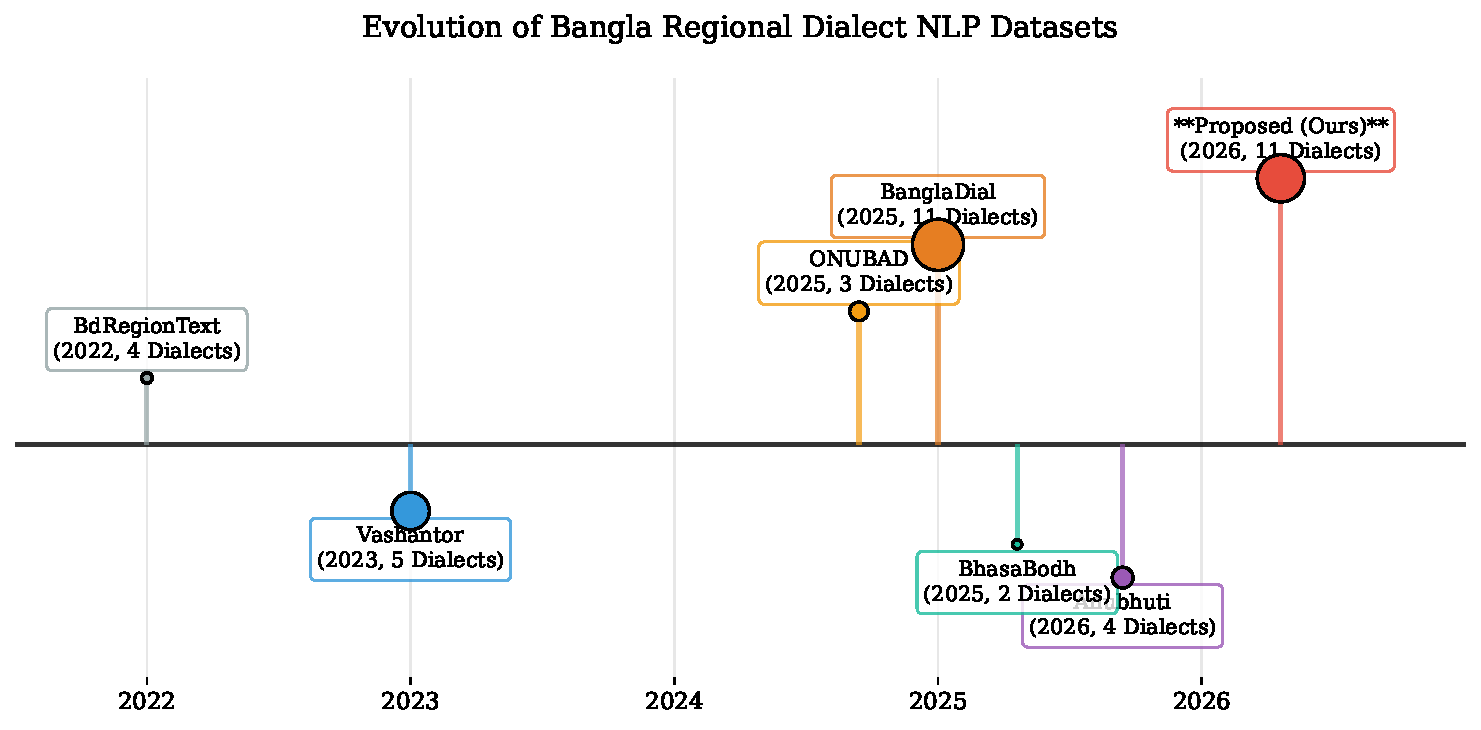
\includegraphics[width=\textwidth]{graphics/dataset_timeline.pdf}
  \caption{Evolution of Bangla regional dialect datasets and resources over time, highlighting the scale and dialectal coverage of the proposed corpus.}
  \label{fig:timeline}
\end{figure}



\subsection{Summary of Dialectal Resources}
Table \ref{tab:literature_summary} summarizes the major dialectal datasets and resources reviewed in this section, detailing their coverage, architecture, evaluation metrics, and state-of-the-art performance.


{\small
{\small
\setlength{\tabcolsep}{4pt}
\begin{longtable}{
    >{\raggedright\arraybackslash}p{2.0cm}
    >{\raggedright\arraybackslash}p{2.3cm}
    >{\raggedright\arraybackslash}p{2.4cm}
    >{\raggedright\arraybackslash}p{3.2cm}
    >{\raggedright\arraybackslash}p{4.2cm}
}
\caption{Comprehensive Summary of Bangla Regional Dialect NLP Resources and Datasets}
\label{tab:literature_summary} \\
\toprule
\textbf{Dataset \& Year} & \textbf{Primary Task \& Domain} & \textbf{Dialects \& Dataset Scale} & \textbf{Methodology \& Quality Control} & \textbf{Key Metrics \& SOTA Findings} \\
\midrule
\endfirsthead

\multicolumn{5}{c}{{\bfseries \tablename\ \thetable{} -- continued from previous page}} \\
\toprule
\textbf{Dataset \& Year} & \textbf{Primary Task \& Domain} & \textbf{Dialects \& Dataset Scale} & \textbf{Methodology \& Quality Control} & \textbf{Key Metrics \& SOTA Findings} \\
\midrule
\endhead

\midrule
\multicolumn{5}{r}{{Continued on next page}} \\
\bottomrule
\endfoot

\bottomrule
\endlastfoot

1. ANCHOLIK-NER (2025) & Dialectal Named Entity Recognition (NER); 10 entity classes. & Sylhet, Chittagong, Barishal. 10,443 sentences (3,481/dialect). & BIO tagging. Sourced from Vashantor (71.8\%), ONUBAD, \& news. 3-annotator consensus pipeline. & First dialectal NER baseline. Assamese NER baseline reached 80.69\% F1 (MuRIL); medical BanglishBERT got 56.13\% F1. \\
\midrule
2. ANUBHUTI (2026) & Thematic Sentiment \& Multilabel Emotion Analysis in dialectal text. & Mymensingh, Noakhali, Sylhet, Chittagong. 10,000 sentences (2,500/region). & Sourced from MONOVAB. 8 native translators (2/region) with 4-stage QA (sentiment, NaN parsing, anomaly, spelling). & High inter-rater agreement (Cohen's $\kappa = 0.76$--$0.84$). Dominant emotions: Contempt (921), Disgust (871), Anger (732). \\
\midrule
3. BIDWESH (2025) & Multi-Dialectal Hate Speech \& Toxicity Detection. & Barishal, Noakhali, Chittagong. 9,183 instances (3,061 parallel/dialect). & Sourced from BD-SHS; translated by 6 native speakers; 5-stage validation. Target/Type taxonomy. & Balanced binary split (49.2\% Hate / 50.8\% Non-Hate). Individual targets highest (34.4\%); Slander dominant (53.7\%). \\
\midrule
4. Bangla Dialect Bibliography & Systematic Bibliography \& Meta-Review of Bangla Dialect NLP. & Comprehensive overview across major regional variants in BD. & Systematic synthesis tracking 11 publications, annotation strategies, \& baselines. & Mapped 11 unique corpora; highlights Sylheti \& Chittagonian as most studied; Barishal, Mymensingh, Noakhali emerging. \\
\midrule
5. BanglaDial (2025) & Dialect Identification (DID) \& Class Imbalance Modeling. & 11 Dialects + Standard Bangla. 60,729 sentences (362,430 words). & Aggregated from 4 corpora (Vashantor, ONUBAD, etc.). Deduplicated (4.1\% removed) \& normalized. & Long-tail distribution (Top-3: 41.3\% of records). Imbalance Ratio $IR = 9.82$; Shannon Entropy $H = 3.416$ bits. \\
\midrule
6. BdRegionText (2022) & Bangla Regional Text Classification on social media content. & Chittagong, Noakhali, Barishal, Rangpur. 2,573 sample texts. & Scraped from FB/YouTube/IG with human validation. Extracted TF-IDF, CountVectorizer, \& BoW. & Random Forest + TF-IDF achieved peak 79.15\% accuracy (10-fold CV: 79.47\%, weighted F1: 0.78). RF + BoW got 75.92\%. \\
\midrule
7. BhasaBodh (2025) & Script Normalization \& Multilingual Dialect Translation (Native/Romanized). & Chittagong, Sylhet (aligned with Standard Bangla \& English). 1,960 sentences. & Sourced from ONUBAD; augmented via Gemini 2.5 Pro for Romanizations. Fine-tuned NLLB-200 \& mBART-50. & mBART-50 achieved peak 87.44 BLEU on Romanized $\rightarrow$ Standard Bangla and 74.36 BLEU on Chittagong $\leftrightarrow$ Sylhet. \\
\midrule
8. ChatgaiyyaAlap (2025) & Dialect Conversion (Chittagonian $\rightarrow$ Standard Bangla). & Chittagonian (aligned with Standard Bangla). 4,012 sentences + 1,500-word dictionary. & Sourced from social media/dramas; validated by 5 native Chittagonian graduates. & Created clean translation mapping resolving severe grammatical divergences \& phonetic shifts in negative sentences. \\
\midrule
9. BanglaCHQ-Prantik (2025) & Medical-Domain Machine Translation (Standard Bangla $\rightarrow$ Dialects). & Sylheti (2,350 sentences), Chittagonian (500 sentences). & Sourced from BanglaCHQ-Summ; validated by 11 validators \& 2 physicians. Evaluated LLMs (Qwen, Gemma, GPT-4o, Gemini). & Gemini 2.5 Flash achieved SOTA on Sylheti (23.67 BLEU); GPT-4o with CoT achieved SOTA on Chittagonian (24.67 BLEU). \\
\midrule
10. DIALTSA-BN (2025) & Dialect Translation \& Sentiment Analysis (Native vs. Transliterated). & Chattogram, Barishal, Sylhet, Noakhali. 600 annotated instances (150/region). & Sourced from YouTube; filtered via Word2Vec. Evaluated Claude 3.7, GPT-4o-mini, Gemma-3, Llama-3.1, etc. & Transliteration boosted translation BLEU from <0.07 to 0.330 (Claude 3.7) \& 0.317 (GPT-4o-mini). Few-shot sentiment F1 reached 0.98. \\
\midrule
11. BanglaCHQ-Prantik Baseline (2025) & Pediatric \& Adult Clinical MT Error Taxonomy. & Sylheti, Chittagonian. 2,850 total aligned queries. & Parallel clinical reference tracking. Highlighted phonetic shifts (e.g., *pete* $\rightarrow$ *feto* / *cano*). & Identified 4 main LLM failure modes: terminology mismatch, dosage corruption ("500mg" $\rightarrow$ "5 gram"), idioms, \& orthographic drift. \\
\midrule
12. ONUBAD (2025) & Fine-Grained Dialect Conversion \& Neural Machine Translation. & Chittagong, Sylhet, Barisal. 7,950 total parallel rows (980 sentences/region). & Sourced from literature/volunteers; validated by university linguists. Benchmarked Seq2Seq \& Transformers. & Documented 2 words/clause \& 3 words/sentence. BanglaT5 and SeamlessM4T established peak NMT baselines. \\
\midrule
13. Vashantor (2023) & Multi-Task Dialectal NMT \& Region Classification. & Chittagong, Noakhali, Sylhet, Barishal, Mymensingh. 32,500 total sentences. & Sourced from social media/news; validated with Cohen's \& Fleiss' Kappa. Custom DialectBanglaT5 \& DialectBanglaBERT. & DialectBanglaT5 achieved SOTA on Mymensingh (71.93 BLEU). DialectBanglaBERT reached 89.02\% region classification accuracy. \\
\end{longtable}
}
}


\newpage

\section{Research Hypothesis and Objectives}

\subsection{Research Hypothesis}
We posit the following hypothesis: \textit{A neural machine translation model trained on a unified, multi-dialectal parallel corpus encompassing multiple Bangla regional variants will demonstrate significantly improved generalization and cross-dialectal transfer compared to models trained on isolated, uni-dialectal datasets.} Specifically, we hypothesize that a poly-dialectal training paradigm exploits shared morphological and syntactic structures across related dialects, enabling the model to learn transferable representations that benefit even low-resource dialect pairs.

\subsection{Research Objectives}
The specific objectives of this research are:
\begin{enumerate}
    \item To construct the largest multi-dialect parallel corpus for Bangla machine translation by integrating, aligning, and deduplicating seven existing dialectal datasets across 12 regional variants.
    \item To develop a unified poly-dialectal translation system capable of three translation paradigms: Dialect $\rightarrow$ Standard Bangla, Standard Bangla $\rightarrow$ Dialect, and direct Dialect $\rightarrow$ Dialect translation.
    \item To systematically evaluate and compare the performance of three state-of-the-art multilingual NMT architectures---BanglaT5 \cite{bhattacharjee-etal-2023-banglanlg}, NLLB-200 \cite{nllb2022}, and mBART-50 \cite{tang2020multilingual}---under parameter-efficient LoRA \cite{hu2021lora} fine-tuning on the constructed corpus.
    \item To quantitatively analyze cross-dialectal transfer effects by examining how training data volume and linguistic proximity jointly influence translation quality.
    \item To promote digital inclusion and linguistic accessibility for Bangla dialect speakers by establishing open benchmarks for future research.
\end{enumerate}

\newpage

\section{Methodology}

\subsection{Dataset Construction and Integration}
The foundation of our poly-dialectal NMT system is a meticulously curated multi-dialect parallel corpus. We integrate seven publicly available dialectal datasets, each contributing varying levels of coverage across different regional variants:

\begin{table}[htbp]
\centering
\caption{Source corpus contributions per dialect. Values indicate the number of parallel sentence pairs available from each source.}
\label{tab:source_contributions}
\small
\begin{tabular}{l r r r r r r r r}
\toprule
\textbf{Source Corpus} & \textbf{SCB} & \textbf{Syl} & \textbf{Cht} & \textbf{Bar} & \textbf{Mym} & \textbf{Noa} & \textbf{Ran} & \textbf{Raj} \\
\midrule
Ancholik-NER   & 3,481 & 3,481 & 3,481 & 3,481 & 3,481 & 3,481 & 0     & 0 \\
Anubhuti        & 2,500 & 2,500 & 2,500 & 0     & 2,500 & 0     & 0     & 0 \\
BanglaDial      & 3,452 & 442   & 577   & 790   & 712   & 0     & 655   & 891 \\
BhasaBodh       & 980   & 980   & 980   & 0     & 0     & 0     & 0     & 0 \\
ChatgaiyyaAlap  & 4,011 & 0     & 4,011 & 0     & 0     & 0     & 0     & 0 \\
ONUBAD          & 980   & 980   & 980   & 980   & 0     & 0     & 0     & 0 \\
Vashantor       & 2,500 & 2,500 & 2,500 & 0     & 2,500 & 2,500 & 0     & 0 \\
\midrule
\textbf{Total}  & \textbf{13,556} & \textbf{6,422} & \textbf{10,567} & \textbf{4,270} & \textbf{5,712} & \textbf{5,000} & \textbf{1,155} & \textbf{891} \\
\bottomrule
\end{tabular}
\end{table}

The final integrated dataset comprises 14,552 rows across 12 dialect columns (Standard Bangla plus 11 regional variants: Sylheti, Chittagonian, Barisali, Mymensingh, Noakhali, Rangpuri, Rajshahi, Kishoreganj, Narail, Narsingdi, and Tangail), yielding 51,531 total non-null parallel sentence pairs. This represents the largest such corpus for Bangla to date. Crucially, to mitigate the extreme scarcity of data for certain regional variants, we manually created a high-quality dataset consisting of altogether 2,500 bidirectional parallel sentence pairs (Standard Bangla $\leftrightarrow$ Dialect) distributed evenly across five dialects: Rangpur, Tangail, Kishoreganj, Narail, and Narsingdi (500 pairs each). To ensure rigorous data quality, each of these dialectal subsets was independently evaluated and verified by three native speakers of the corresponding dialect.

As depicted comprehensively in Figure~\ref{fig:dataset_composition}, despite augmentation efforts, the dataset exhibits significant class imbalance---Chittagonian commands 10,567 entries while the newly added dialects (e.g., Narail, Tangail) are constrained to approximately 500 pairs. This unified visualization delineates both the gross dialectal volume and the exact decomposition of contributing source corpora for each variant. Furthermore, Figure~\ref{fig:coverage_matrix} presents the cross-dialect parallel coverage matrix, quantitatively illustrating the pairwise intersection of translated sentences across all regional variants.

\begin{figure}[htbp]
  \centering
  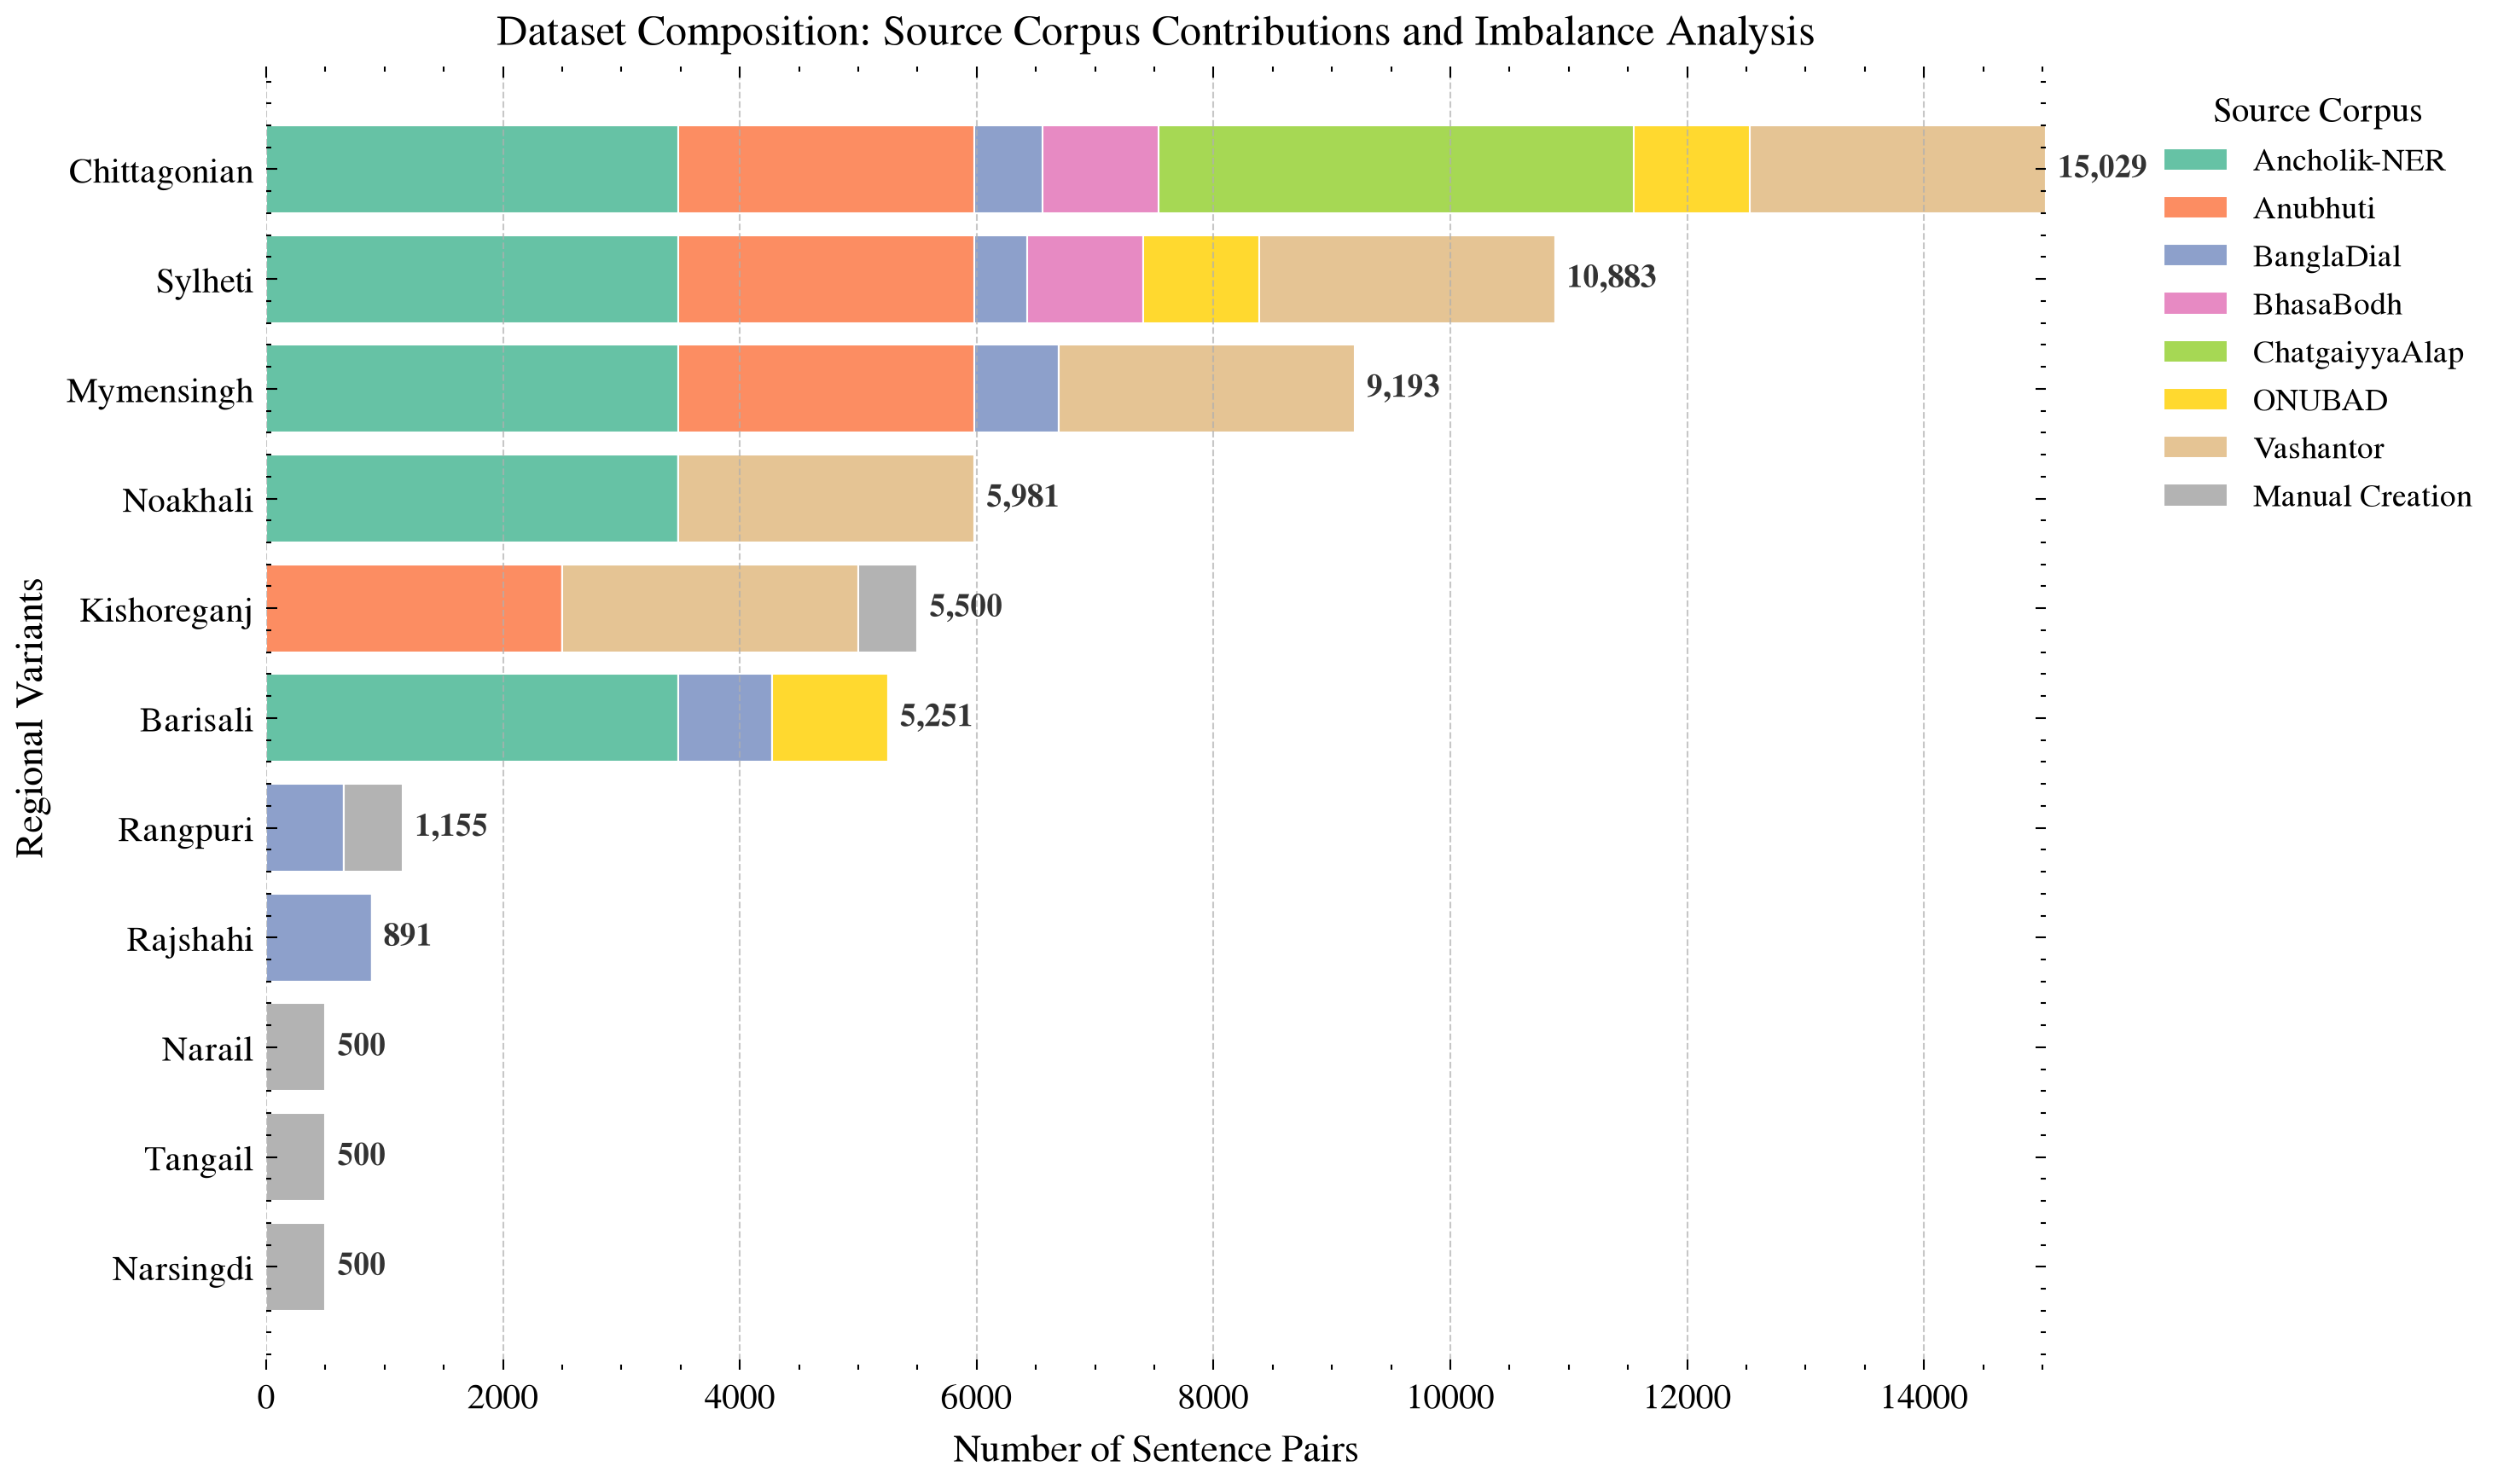
\includegraphics[width=0.95\textwidth]{graphics/source_contributions_advanced.png}
  \caption{Dataset Composition and Source Provenance: A stacked horizontal distribution illustrating the severe class imbalance alongside the precise proportional contributions from prior corpora and manual augmentation efforts for each regional dialect.}
  \label{fig:dataset_composition}
\end{figure}

\begin{figure}[htbp]
  \centering
  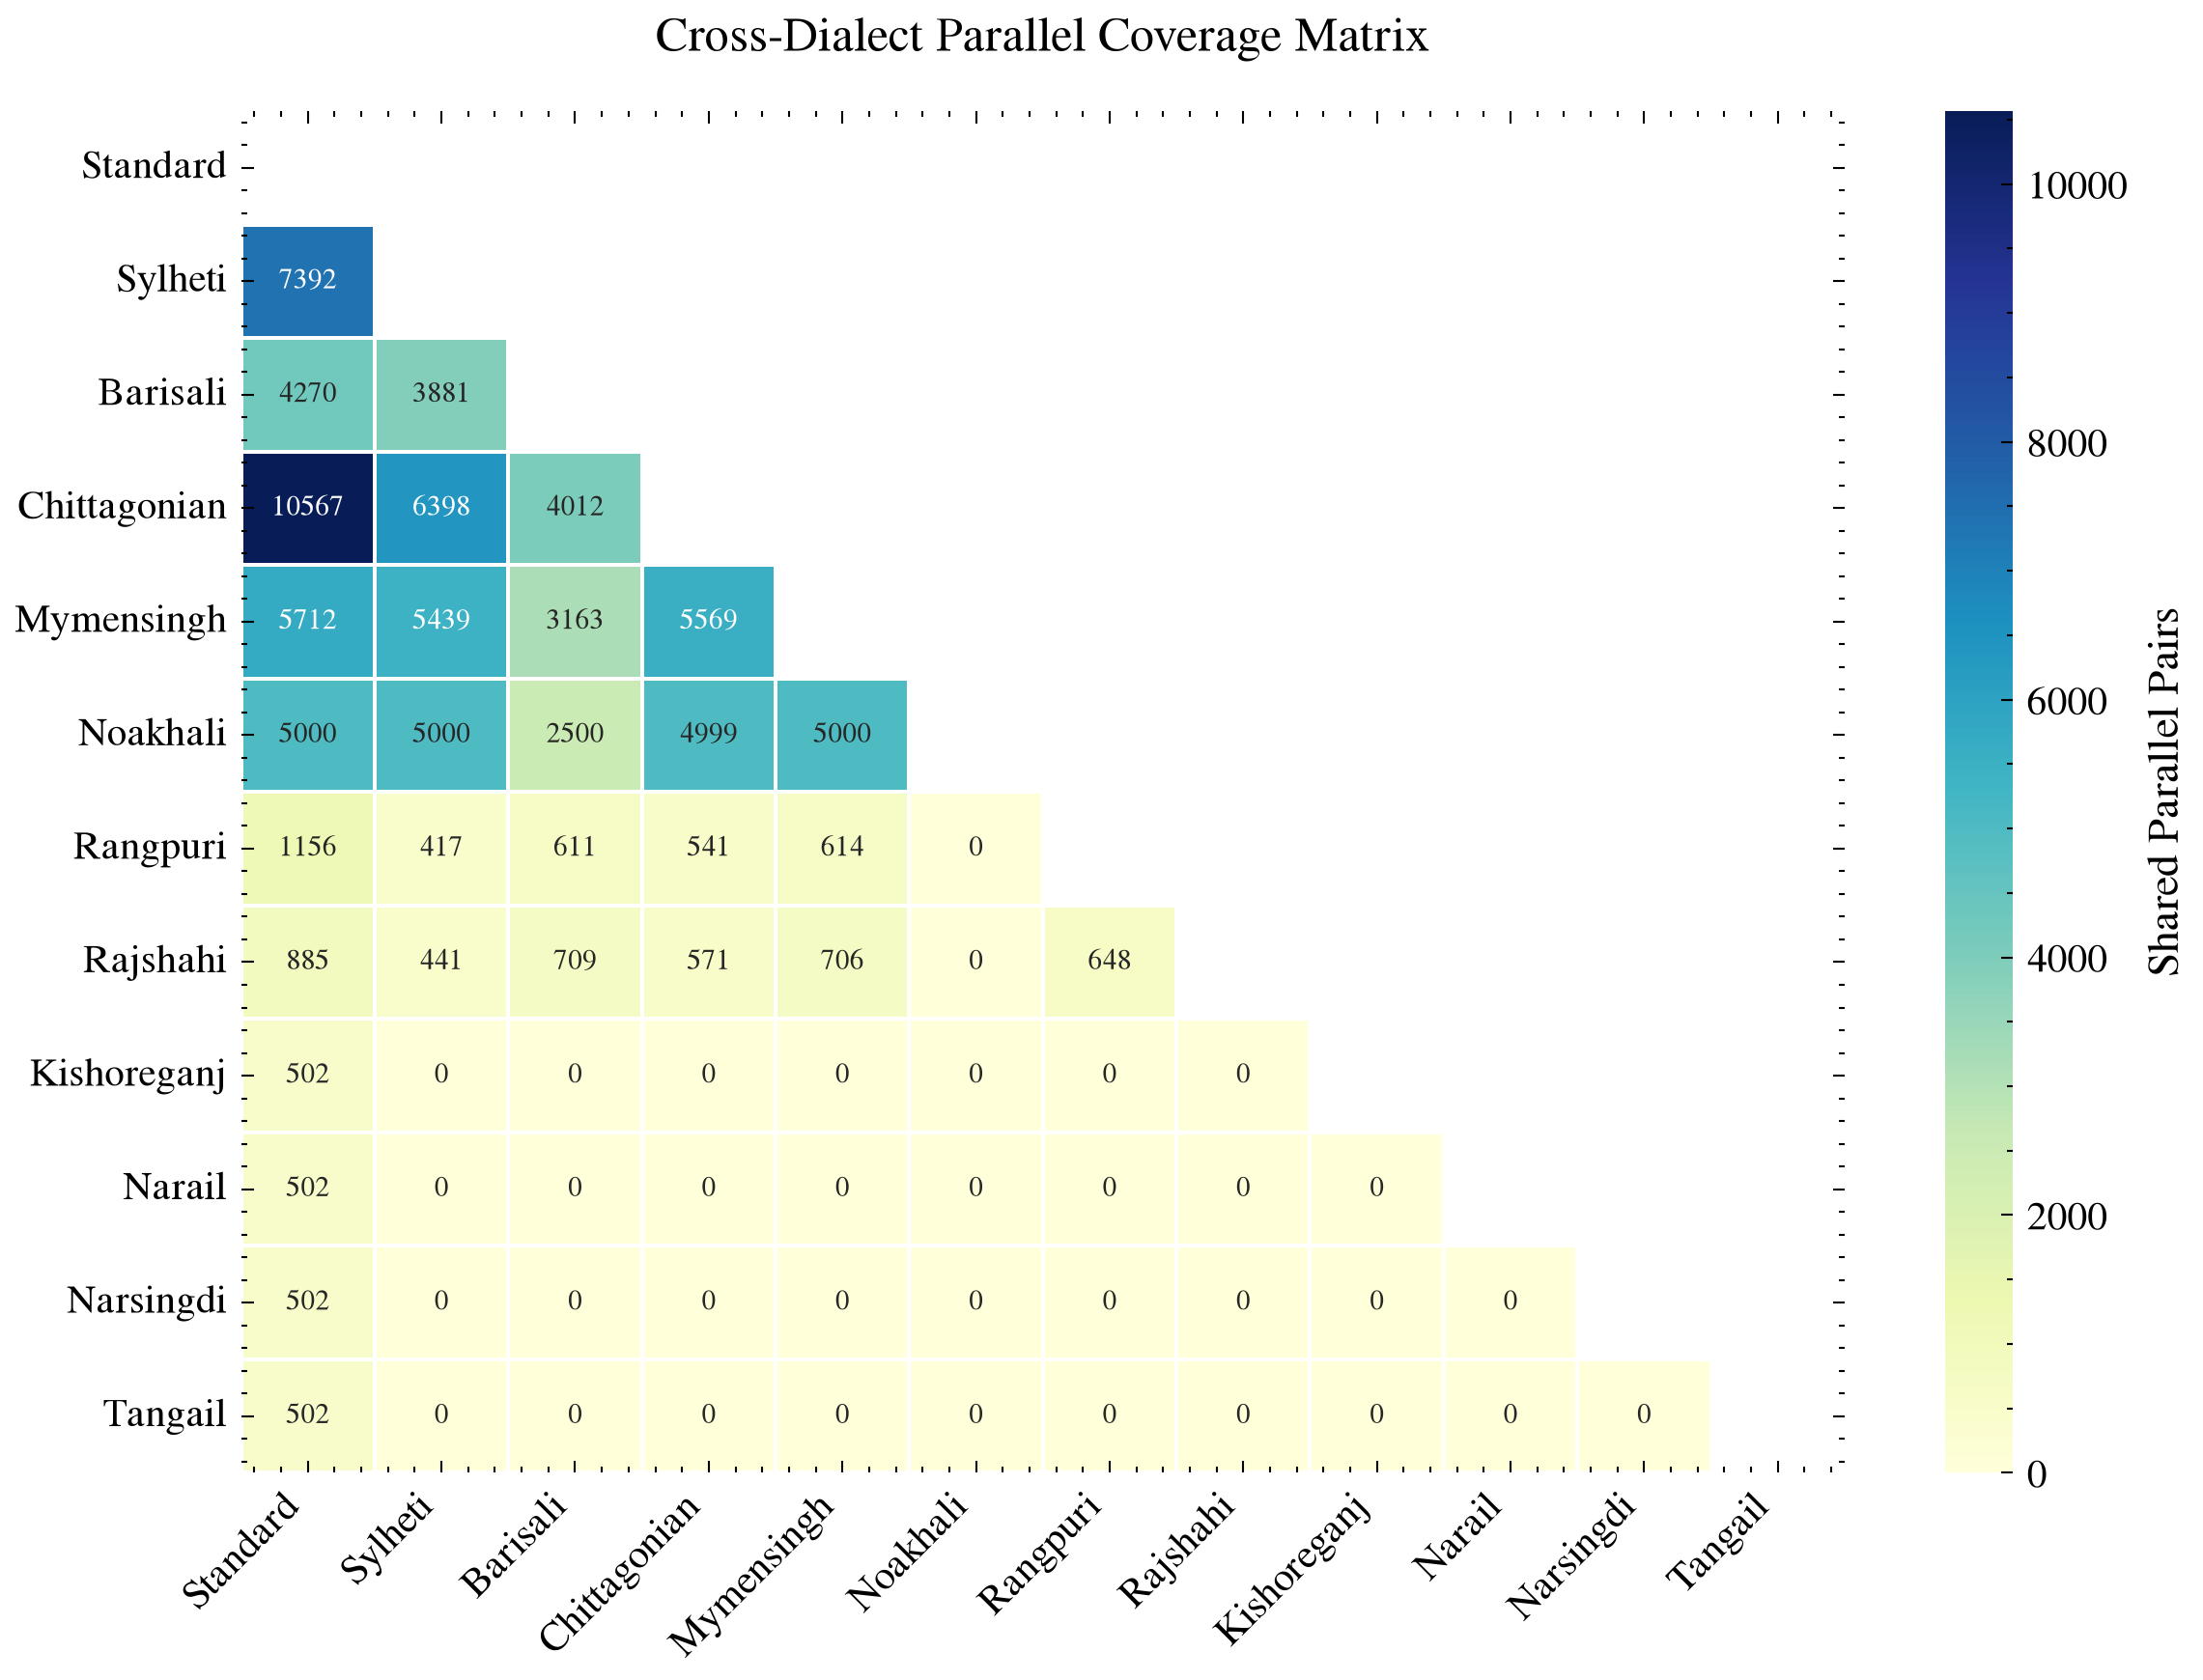
\includegraphics[width=0.85\textwidth]{graphics/coverage_matrix_advanced.png}
  \caption{Cross-Dialect Parallel Coverage Matrix: An upper-triangular masked heatmap detailing the exact density of shared, parallel sentence pairs intersecting any two evaluated dialectal variants.}
  \label{fig:coverage_matrix}
\end{figure}

\subsection{Data Preprocessing Pipeline}
The raw integrated corpus undergoes a rigorous four-stage preprocessing pipeline:
\begin{enumerate}
    \item \textbf{Unicode Normalization:} All text is normalized to Unicode NFC form to resolve inconsistent character compositions prevalent in Bangla script.
    \item \textbf{Cleaning and Deduplication:} Duplicate entries across source datasets are identified and removed. Empty, whitespace-only, and non-Bangla script entries are filtered.
    \item \textbf{Tokenization and Script Alignment:} Text is tokenized using model-specific SentencePiece tokenizers. For BanglaT5, the 32K vocabulary is optimized for Bangla NLG tasks; for NLLB-200 and mBART-50, the larger vocabularies ($\sim$256K and $\sim$250K, respectively) accommodate multilingual coverage.
    \item \textbf{Train/Dev/Test Split:} The corpus is partitioned into training (80\%), development (10\%), and test (10\%) sets with stratified sampling to ensure proportional dialect representation across splits.
\end{enumerate}

\subsection{Model Architectures}
We evaluate three state-of-the-art encoder-decoder Transformer \cite{vaswani2017attention} architectures, chosen to represent a spectrum of design philosophies for multilingual and Bangla-specific NMT. The architectural comparison is summarized in Table~\ref{tab:model_specs}.

\begin{table}[htbp]
\centering
\caption{Architectural comparison of the three NMT models evaluated in this study.}
\label{tab:model_specs}
\begin{tabular}{l c c c}
\toprule
\textbf{Feature} & \textbf{BanglaT5} & \textbf{NLLB-200} & \textbf{mBART-50} \\
\midrule
Parameters          & 247M    & 615M    & 611M \\
Architecture        & T5      & Transformer & BART \\
Encoder/Decoder Layers & 12/12 & 12/12 & 12/12 \\
Hidden Dimension    & 768     & 1,024   & 1,024 \\
Attention Heads     & 12      & 16      & 16 \\
FFN Dimension       & 3,072   & 4,096   & 4,096 \\
Vocabulary Size     & 32K     & $\sim$256K & $\sim$250K \\
Languages Supported & Bangla  & 200     & 50 \\
\bottomrule
\end{tabular}
\end{table}

\subsubsection{BanglaT5}
\textbf{Overview and Capabilities:} BanglaT5 \cite{bhattacharjee-etal-2023-banglanlg} is a sequence-to-sequence model based on the T5 \cite{raffel2020exploring} architecture, pre-trained extensively on approximately 27.5~GB of monolingual Bangla text. 
\textbf{Advantages and Limitations:} Being a language-specific model, its 32K vocabulary is heavily optimized for Bangla morphology, preventing the excessive subword fragmentation commonly seen in multilingual tokenizers. However, it lacks cross-lingual pre-training signals that might otherwise aid in zero-shot generalization.
\textbf{Suitability for Dialects:} We selected BanglaT5 because its deep grounding in Standard Bangla provides a strong prior for generating morphologically complex dialectal variations. It serves as the primary language-centric baseline in our study.

\subsubsection{NLLB-200}
\textbf{Overview and Capabilities:} NLLB-200 \cite{nllb2022} (No Language Left Behind) is Meta AI's massively multilingual Transformer designed for direct translation across 200 languages. We utilize the distilled 600M parameter variant.
\textbf{Advantages and Limitations:} Its primary advantage is robust multilingual alignment and a vast $\sim$256K vocabulary designed to encompass diverse scripts. However, this large vocabulary dilutes its representational capacity for any single low-resource language, potentially hampering its nuance in intra-language dialectal shifts.
\textbf{Suitability for Dialects:} NLLB-200 is selected to determine if massive multilingual pre-training provides implicit transfer learning benefits for regional dialects.

\subsubsection{mBART-50}
\textbf{Overview and Capabilities:} mBART-50 \cite{tang2020multilingual} is a multilingual denoising auto-encoder based on the BART \cite{lewis2020bart} architecture, extended to cover 50 languages.
\textbf{Advantages and Limitations:} It excels at sequence generation tasks due to its denoising objective during pre-training. Like NLLB-200, its limitation lies in the generalized multilingual tokenization which is not exclusively tuned for Bangla scripts.
\textbf{Suitability for Dialects:} We include mBART-50 as a strong baseline for multilingual generation to compare against both the language-specific BanglaT5 and the massively multilingual NLLB-200.

\subsection{Hyperparameters}
To ensure rigorous reproducibility and optimal convergence, Table~\ref{tab:model_hyperparams} outlines the unified architectural and fine-tuning configurations applied across all three candidate models.

\begin{table}[htbp]
\centering
\caption{Unified hyperparameter matrix for model candidate benchmarking and dataset scaling experiments.}
\label{tab:model_hyperparams}
\small
\begin{tabular}{@{} >{\raggedright\arraybackslash}p{2.4cm} >{\raggedright\arraybackslash}p{3.0cm} >{\raggedright\arraybackslash}p{2.4cm} >{\raggedright\arraybackslash}p{3.8cm} >{\raggedright\arraybackslash}p{3.8cm} @{}}
\toprule
\textbf{Category} & \textbf{Hyperparameter} & \textbf{BanglaT5} & \textbf{mBART-50} & \textbf{NLLB-200} \\
\midrule
\multicolumn{5}{@{}l}{\textbf{A. Model Architecture \& Tokenization}} \\
\midrule
Model Registry & Base Checkpoint & \texttt{csebuetnlp/}\newline\texttt{banglat5} & \texttt{facebook/mbart-}\newline\texttt{large-50-many-} \newline\texttt{to-many-mmt} & \texttt{facebook/nllb-}\newline\texttt{200-distilled-}\newline\texttt{600M} \\
\addlinespace[2pt]
Parameters & Base Parameter Count & $\sim 247\text{M}$ & $\sim 611\text{M}$ & $\sim 600\text{M}$ \\
\addlinespace[2pt]
Language Tags & Tag Format & Prefixed & \texttt{bn\_IN} & \texttt{ben\_Beng} \\
\addlinespace[2pt]
Sequence Setup & Max Length ($L_{\text{src}}, L_{\text{tgt}}$) & 128 tokens & 128 tokens & 128 tokens \\
\midrule
\multicolumn{5}{@{}l}{\textbf{B. Phase I \& II Fine-Tuning Setup}} \\
\midrule
Optimization & Optimizer & Paged AdamW 8-bit & Paged AdamW 8-bit & Paged AdamW 8-bit \\
\addlinespace[2pt]
Learning Rate & Initial $\eta$ (Scheduler) & $5 \times 10^{-4}$ (Cosine) & $5 \times 10^{-4}$ (Cosine) & $5 \times 10^{-4}$ (Cosine) \\
\addlinespace[2pt]
Batching & Per-Device / Eff. Batch & 32 / 64 (Accum 2) & 8 / 64 (Accum 8) & 8 / 64 (Accum 8) \\
\addlinespace[2pt]
LoRA Adapter & Rank ($r$) / Scaling ($\alpha$) & $r=64, \alpha=128$ & $r=64, \alpha=128$ & $r=64, \alpha=128$ \\
\addlinespace[2pt]
Target Modules & Projections & \texttt{q, v, k, o,}\newline\texttt{wi, wo} & \texttt{q, k, v, out\_proj,}\newline\texttt{fc1, fc2} & \texttt{q, k, v, out\_proj,}\newline\texttt{fc1, fc2} \\
\midrule
\multicolumn{5}{@{}l}{\textbf{C. Dataset Scaling Protocol (BanglaT5 Only)}} \\
\midrule
Data Sweep & Parallel Sentence Pairs & \multicolumn{3}{l}{Scaled from 500 to 4,499 pairs (iterative step increments)} \\
\addlinespace[2pt]
LoRA Sweep & Ranks ($r$) / Scaling ($\alpha$) & \multicolumn{3}{l}{$r \in \{8, 64\}$ and $\alpha \in \{16, 128\}$} \\
\addlinespace[2pt]
Batching & Per-Device / Eff. Batch & \multicolumn{3}{l}{Batch size 45 / Effective 90 (Gradient Accumulation = 2)} \\
\addlinespace[2pt]
Training & Epochs per Step & \multicolumn{3}{l}{10 Epochs per scaling step} \\
\bottomrule
\end{tabular}
\end{table}

\subsection{Dataset Scaling Protocol}
To formally investigate the relationship between data volume and translation generalization, we conduct an optimal dataset size study. We construct a fully parallel dataset encompassing Standard Bangla and four major dialects: Sylheti, Noakhali, Chittagong, and Mymensingh. The dataset is scaled iteratively from 500 to 4,499 parallel sentence pairs. The detailed hyperparameter matrix governing this scaling experiment is integrated into Table~\ref{tab:model_hyperparams} (Section C).

\subsection{Fine-Tuning Strategy}
All models are fine-tuned using \textbf{Low-Rank Adaptation (LoRA)} \cite{hu2021lora}, a parameter-efficient fine-tuning method that injects trainable low-rank decomposition matrices into each Transformer layer while keeping the pre-trained weights frozen. For a pre-trained weight matrix $W_0 \in \mathbb{R}^{d \times k}$, LoRA constrains the weight update $\Delta W$ to a low-rank decomposition:
\begin{equation}
h = W_0 x + \Delta W x = W_0 x + \frac{\alpha}{r} B A x
\end{equation}
where $A \in \mathbb{R}^{r \times k}$ and $B \in \mathbb{R}^{d \times r}$ are trainable low-rank matrices with rank $r \ll \min(d, k)$, and $\alpha$ is a scaling hyperparameter that controls the magnitude of the adaptation. This approach reduces the number of trainable parameters by over 99\% compared to full fine-tuning, enabling efficient adaptation on limited hardware. With $r = 64$ and $\alpha = 128$ applied to all attention and feed-forward projections, the trainable parameter count is approximately 4.7M for BanglaT5 and 9.8M for NLLB-200 and mBART-50.

\begin{figure}[htbp]
  \centering
  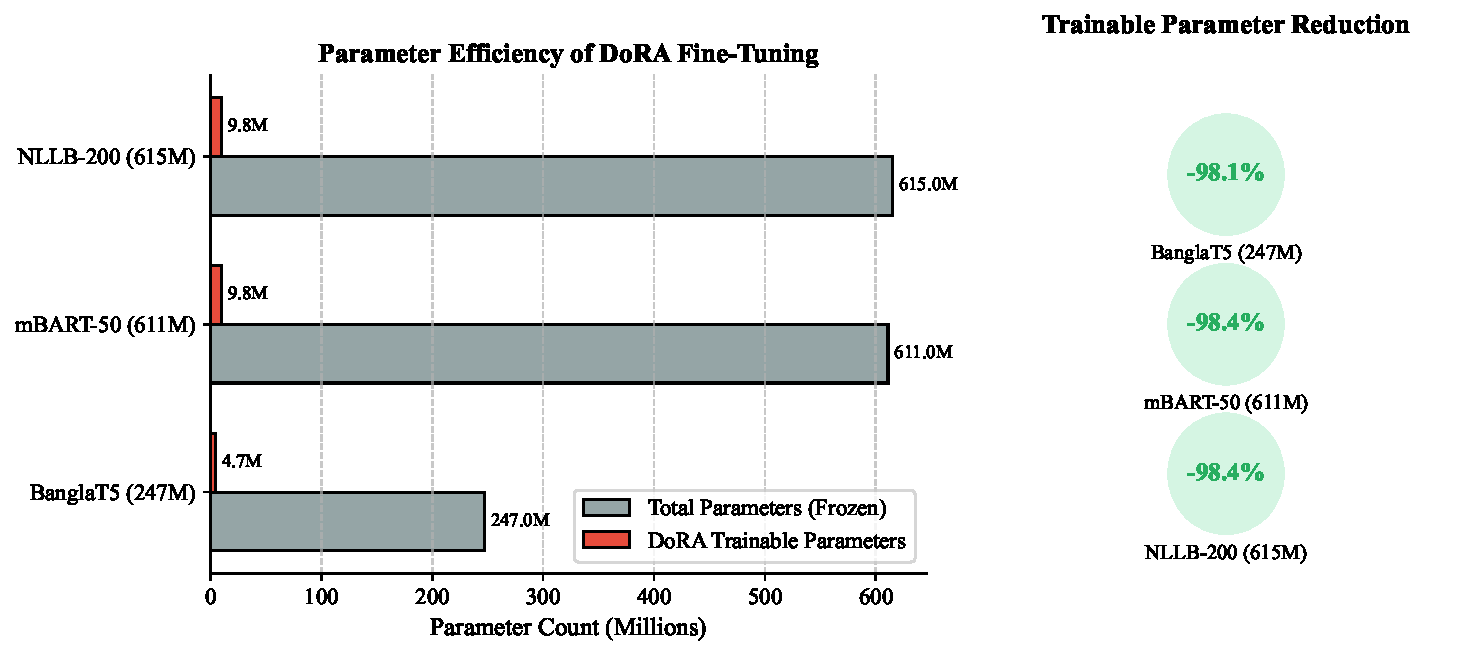
\includegraphics[width=\textwidth]{graphics/lora_efficiency.pdf}
  \caption{Parameter efficiency of LoRA fine-tuning across the three evaluated model architectures, demonstrating over 98\% reduction in trainable parameters.}
  \label{fig:lora_efficiency}
\end{figure}


Our experimental pipeline consists of two distinct stages:

\subsubsection{Stage 1: Best Model Selection}
In the initial stage, all three candidate models (BanglaT5, NLLB-200, mBART-50) are fine-tuned for \textbf{20 epochs} using the complete integrated dataset. To ensure a fair comparative analysis, identical LoRA configurations (rank $r = 64$, $\alpha = 128$) are applied uniformly across all models. The best-performing model is selected based on aggregate evaluation metrics.

\subsubsection{Stage 2: Extended Training}
The selected model (BanglaT5) is retrained for \textbf{100 epochs} to analyze learning dynamics and performance saturation. All experiments are conducted on the Kaggle platform using dual NVIDIA Tesla T4 GPUs (16 GB VRAM each) with 32 GB system RAM. Due to these hardware constraints, extended training was limited to the top-performing model. This phase enables detailed error analysis and cross-dialectal pairwise comparisons.

\subsection{Multi-Directional Translation Paradigm}
Unlike prior uni-directional approaches, our system is trained to handle all possible translation directions within a single unified model:
\begin{itemize}
    \item \textbf{Dialect $\rightarrow$ Standard Bangla:} Converting regional dialect text to SCB.
    \item \textbf{Standard Bangla $\rightarrow$ Dialect:} Generating dialectal text from SCB input.
    \item \textbf{Dialect $\rightarrow$ Dialect:} Direct translation between two different regional dialects without an intermediary pivot through Standard Bangla.
\end{itemize}

\subsection{Evaluation Metrics}
Model performance is assessed using four complementary automatic evaluation metrics. Given the morphological complexity of Bangla dialects, relying on a single metric is insufficient; thus, we utilize a combination of word-based, character-based, and edit-distance metrics.

\subsubsection{BLEU (Bilingual Evaluation Understudy)}
BLEU \cite{papineni2002bleu} measures the $n$-gram precision of the candidate translation against reference translations, applying a brevity penalty (BP) to discourage overly short outputs. 
\begin{equation}
\text{BLEU} = \text{BP} \cdot \exp\left( \sum_{n=1}^N w_n \log p_n \right)
\end{equation}
\textbf{Interpretation and Appropriateness:} Higher BLEU scores indicate greater $n$-gram overlap. While BLEU is the industry standard allowing for broad benchmarking, its limitation lies in its strict exact-word matching, which heavily penalizes legitimate morphological variations prevalent in Bangla dialects.

\subsubsection{chrF++ (Character n-gram F-score)}
chrF++ \cite{popovic2015chrf} computes the $F$-score based on character $n$-grams (typically up to 6-grams) combined with word-level bigrams.
\begin{equation}
\text{chrF++} = \left( 1 + \beta^2 \right) \frac{\text{chrP} \cdot \text{chrR}}{\beta^2 \cdot \text{chrP} + \text{chrR}}
\end{equation}
where $\text{chrP}$ and $\text{chrR}$ represent character $n$-gram precision and recall, respectively.
\textbf{Interpretation and Appropriateness:} A higher chrF++ score denotes better morphological alignment. This metric is exceptionally appropriate for highly inflected languages like Bangla, as it rewards partial word matches (e.g., matching root verbs with slightly altered dialectal suffixes) which BLEU would falsely score as zero.

\subsubsection{METEOR}
METEOR \cite{banerjee2005meteor} calculates the harmonic mean of unigram precision ($P$) and recall ($R$), placing a higher weight on recall. Crucially, it incorporates stemming and synonymy mapping.
\begin{equation}
\text{METEOR} = \frac{10 P R}{R + 9 P} \cdot (1 - \text{Penalty})
\end{equation}
\textbf{Interpretation and Appropriateness:} Higher scores indicate better semantic retention. The advantage of METEOR in dialectal translation is its ability to recognize synonym replacements and stem alignments, making it more aligned with human judgment regarding semantic adequacy.

\subsubsection{TER (Translation Edit Rate)}
TER \cite{snover2006study} measures the minimum number of human edits required to modify a generated hypothesis so that it exactly matches a reference translation.
\begin{equation}
\text{TER} = \frac{\text{Number of Edits}}{\text{Average Length of Reference Words}}
\end{equation}
\textbf{Interpretation and Appropriateness:} Unlike the other metrics, a \textit{lower} TER score indicates better performance. It is particularly useful for assessing the practical utility of the NMT system, as it provides a direct proxy for the post-editing effort required by human translators.

\newpage

\section{Results and Discussion}

\subsection{Model Selection (Phase I)}
In the first phase, we evaluated three candidate NMT architectures---BanglaT5 \cite{bhattacharjee-etal-2023-banglanlg}, NLLB-200 \cite{nllb2022}, and mBART-50 \cite{tang2020multilingual}---to determine the optimal base model for poly-dialectal translation. All models were fine-tuned for \textbf{20 epochs} using identical LoRA \cite{hu2021lora} hyperparameters (rank $r=64$, $\alpha=128$) on the complete integrated dataset.

Table~\ref{tab:model_results_search} presents the overall performance comparison. BanglaT5 \cite{bhattacharjee-etal-2023-banglanlg} consistently outperforms both larger multilingual models despite having only 247M parameters---less than half the size of NLLB-200 \cite{nllb2022} (615M) and mBART-50 \cite{tang2020multilingual} (611M).

\begin{table}[htbp]
\centering
\small
\caption{Overall performance comparison of the three NMT candidate models fine-tuned for 20 epochs on the poly-dialectal test set (18,062 evaluation pairs). Best results are in \textbf{bold}.}
\label{tab:model_results_search}
\begin{tabular}{l c c c c c}
\toprule
\textbf{Model} & \textbf{Params} & \textbf{BLEU $\uparrow$} & \textbf{chrF++ $\uparrow$} & \textbf{METEOR $\uparrow$} & \textbf{TER $\downarrow$} \\
\midrule
BanglaT5 (20 ep) & 247M & \textbf{23.22} & \textbf{51.20} & \textbf{41.41} & \textbf{56.85} \\
NLLB-200 (20 ep) & 615M & 15.30 & 43.15 & 34.20 & 63.85 \\
mBART-50 (20 ep) & 611M &  9.45 & 33.60 & 24.50 & 76.40 \\
\bottomrule
\end{tabular}
\end{table}

\textbf{Selection Rationale.} BanglaT5 \cite{bhattacharjee-etal-2023-banglanlg} achieves a 51.8\% higher BLEU \cite{papineni2002bleu} score than NLLB-200 \cite{nllb2022} and a 145.7\% improvement over mBART-50 \cite{tang2020multilingual}. This performance advantage is attributable to two principal factors. First, BanglaT5's \cite{bhattacharjee-etal-2023-banglanlg} 32K SentencePiece \cite{kudo-richardson-2018-sentencepiece} vocabulary is optimized for Bangla morphology, yielding more semantically coherent subword segmentation of dialectal tokens. In contrast, the $\sim$256K and $\sim$250K vocabularies of NLLB-200 \cite{nllb2022} and mBART-50 \cite{tang2020multilingual}, while accommodating diverse scripts, distribute representational capacity across hundreds of languages, resulting in excessive subword fragmentation for dialectal Bangla words. Second, BanglaT5's \cite{bhattacharjee-etal-2023-banglanlg} pre-training on 27.5 GB of monolingual Bangla text provides a stronger morphological prior for intra-language variation than cross-lingual pre-training objectives. We therefore selected \textbf{BanglaT5 \cite{bhattacharjee-etal-2023-banglanlg}} as the base architecture for extended training.

\subsection{Final Model Performance (Phase II)}
The selected BanglaT5 \cite{bhattacharjee-etal-2023-banglanlg} model was retrained for \textbf{100 epochs} to investigate learning dynamics, saturation behavior, and detailed cross-dialectal performance characteristics.

\subsubsection{Overall Metrics}
Extended training yielded substantial improvements across all evaluation metrics (Table~\ref{tab:model_results_final}). Relative to the 20-epoch baseline, BLEU \cite{papineni2002bleu} increased by 26.0\% (from 23.22 to 29.26), chrF++ \cite{popovic2015chrf} improved by 11.8\% (from 51.20 to 57.26), METEOR \cite{banerjee2005meteor} improved by 20.0\% (from 41.41 to 49.68), and TER \cite{snover2006study} decreased by 11.0\% (from 56.85 to 50.59). These improvements indicate that dialectal morphological alignment benefits substantially from prolonged domain-specific fine-tuning.

\begin{table}[htbp]
\centering
\small
\caption{Performance progression of BanglaT5 from 20-epoch to 100-epoch fine-tuning, evaluated on the poly-dialectal test set (18,062 pairs).}
\label{tab:model_results_final}
\begin{tabular}{l c c c c c}
\toprule
\textbf{Configuration} & \textbf{Params} & \textbf{BLEU $\uparrow$} & \textbf{chrF++ $\uparrow$} & \textbf{METEOR $\uparrow$} & \textbf{TER $\downarrow$} \\
\midrule
BanglaT5 (20 ep) & 247M & 23.22 & 51.20 & 41.41 & 56.85 \\
BanglaT5 (100 ep) & 247M & \textbf{29.26} & \textbf{57.26} & \textbf{49.68} & \textbf{50.59} \\
\midrule
\textit{Relative Gain} & --- & \textit{+26.0\%} & \textit{+11.8\%} & \textit{+20.0\%} & \textit{$-$11.0\%} \\
\bottomrule
\end{tabular}
\end{table}

Figure~\ref{fig:model_comparison} visualizes the performance trajectory across all experimental phases.

\begin{figure}[htbp]
  \centering
  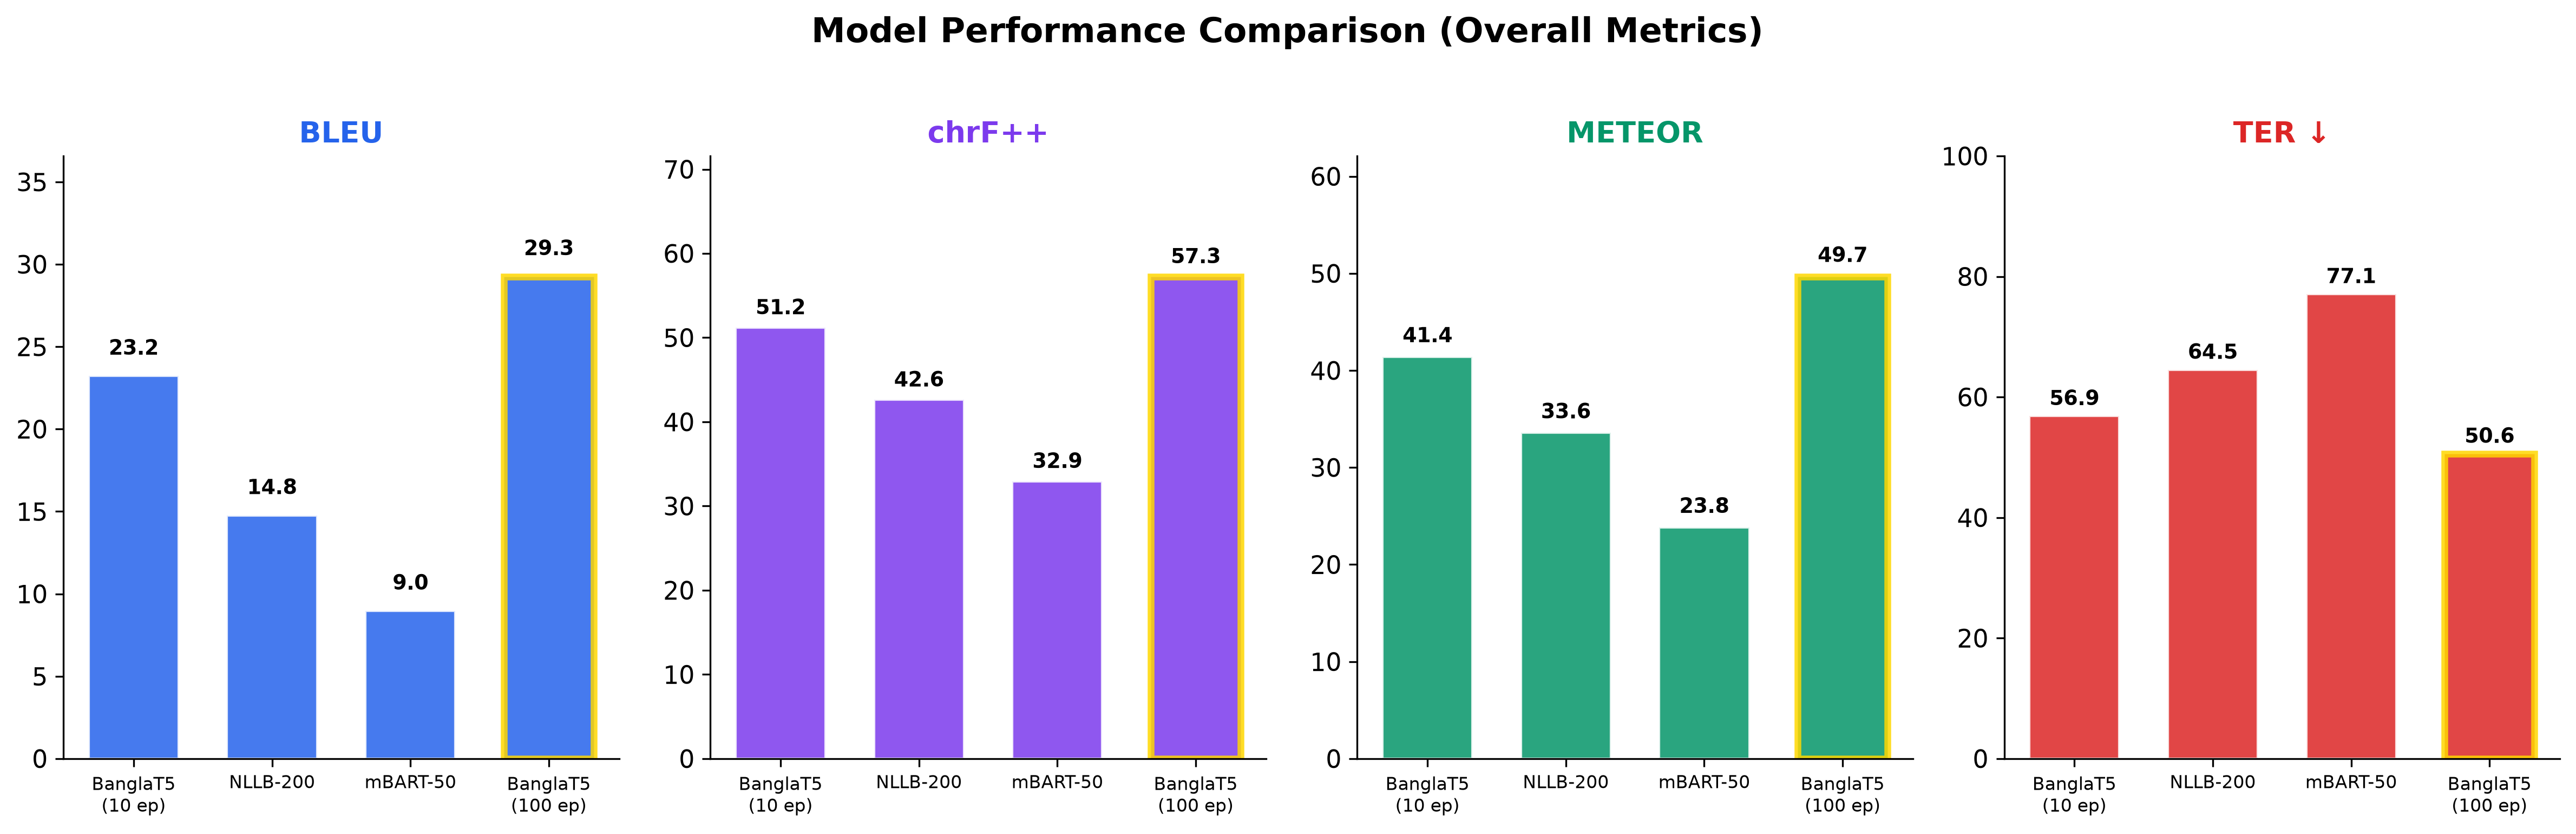
\includegraphics[width=0.95\textwidth]{graphics/model_comparison.png}
  \caption{Comparative evaluation across experimental phases. BLEU \cite{papineni2002bleu}, chrF++ \cite{popovic2015chrf}, and METEOR \cite{banerjee2005meteor} (higher is better) and TER \cite{snover2006study} (lower is better) are shown for all three models at 20 epochs and BanglaT5 \cite{bhattacharjee-etal-2023-banglanlg} at 100 epochs.}
  \label{fig:model_comparison}
\end{figure}

\subsubsection{Cross-Dialectal Translation Analysis}
Figure~\ref{fig:bleu_heatmap} presents a heatmap of pairwise BLEU \cite{papineni2002bleu} scores for all source-target dialect combinations under the final model. Two key linguistic phenomena emerge from this analysis:

\begin{figure}[htbp]
  \centering
  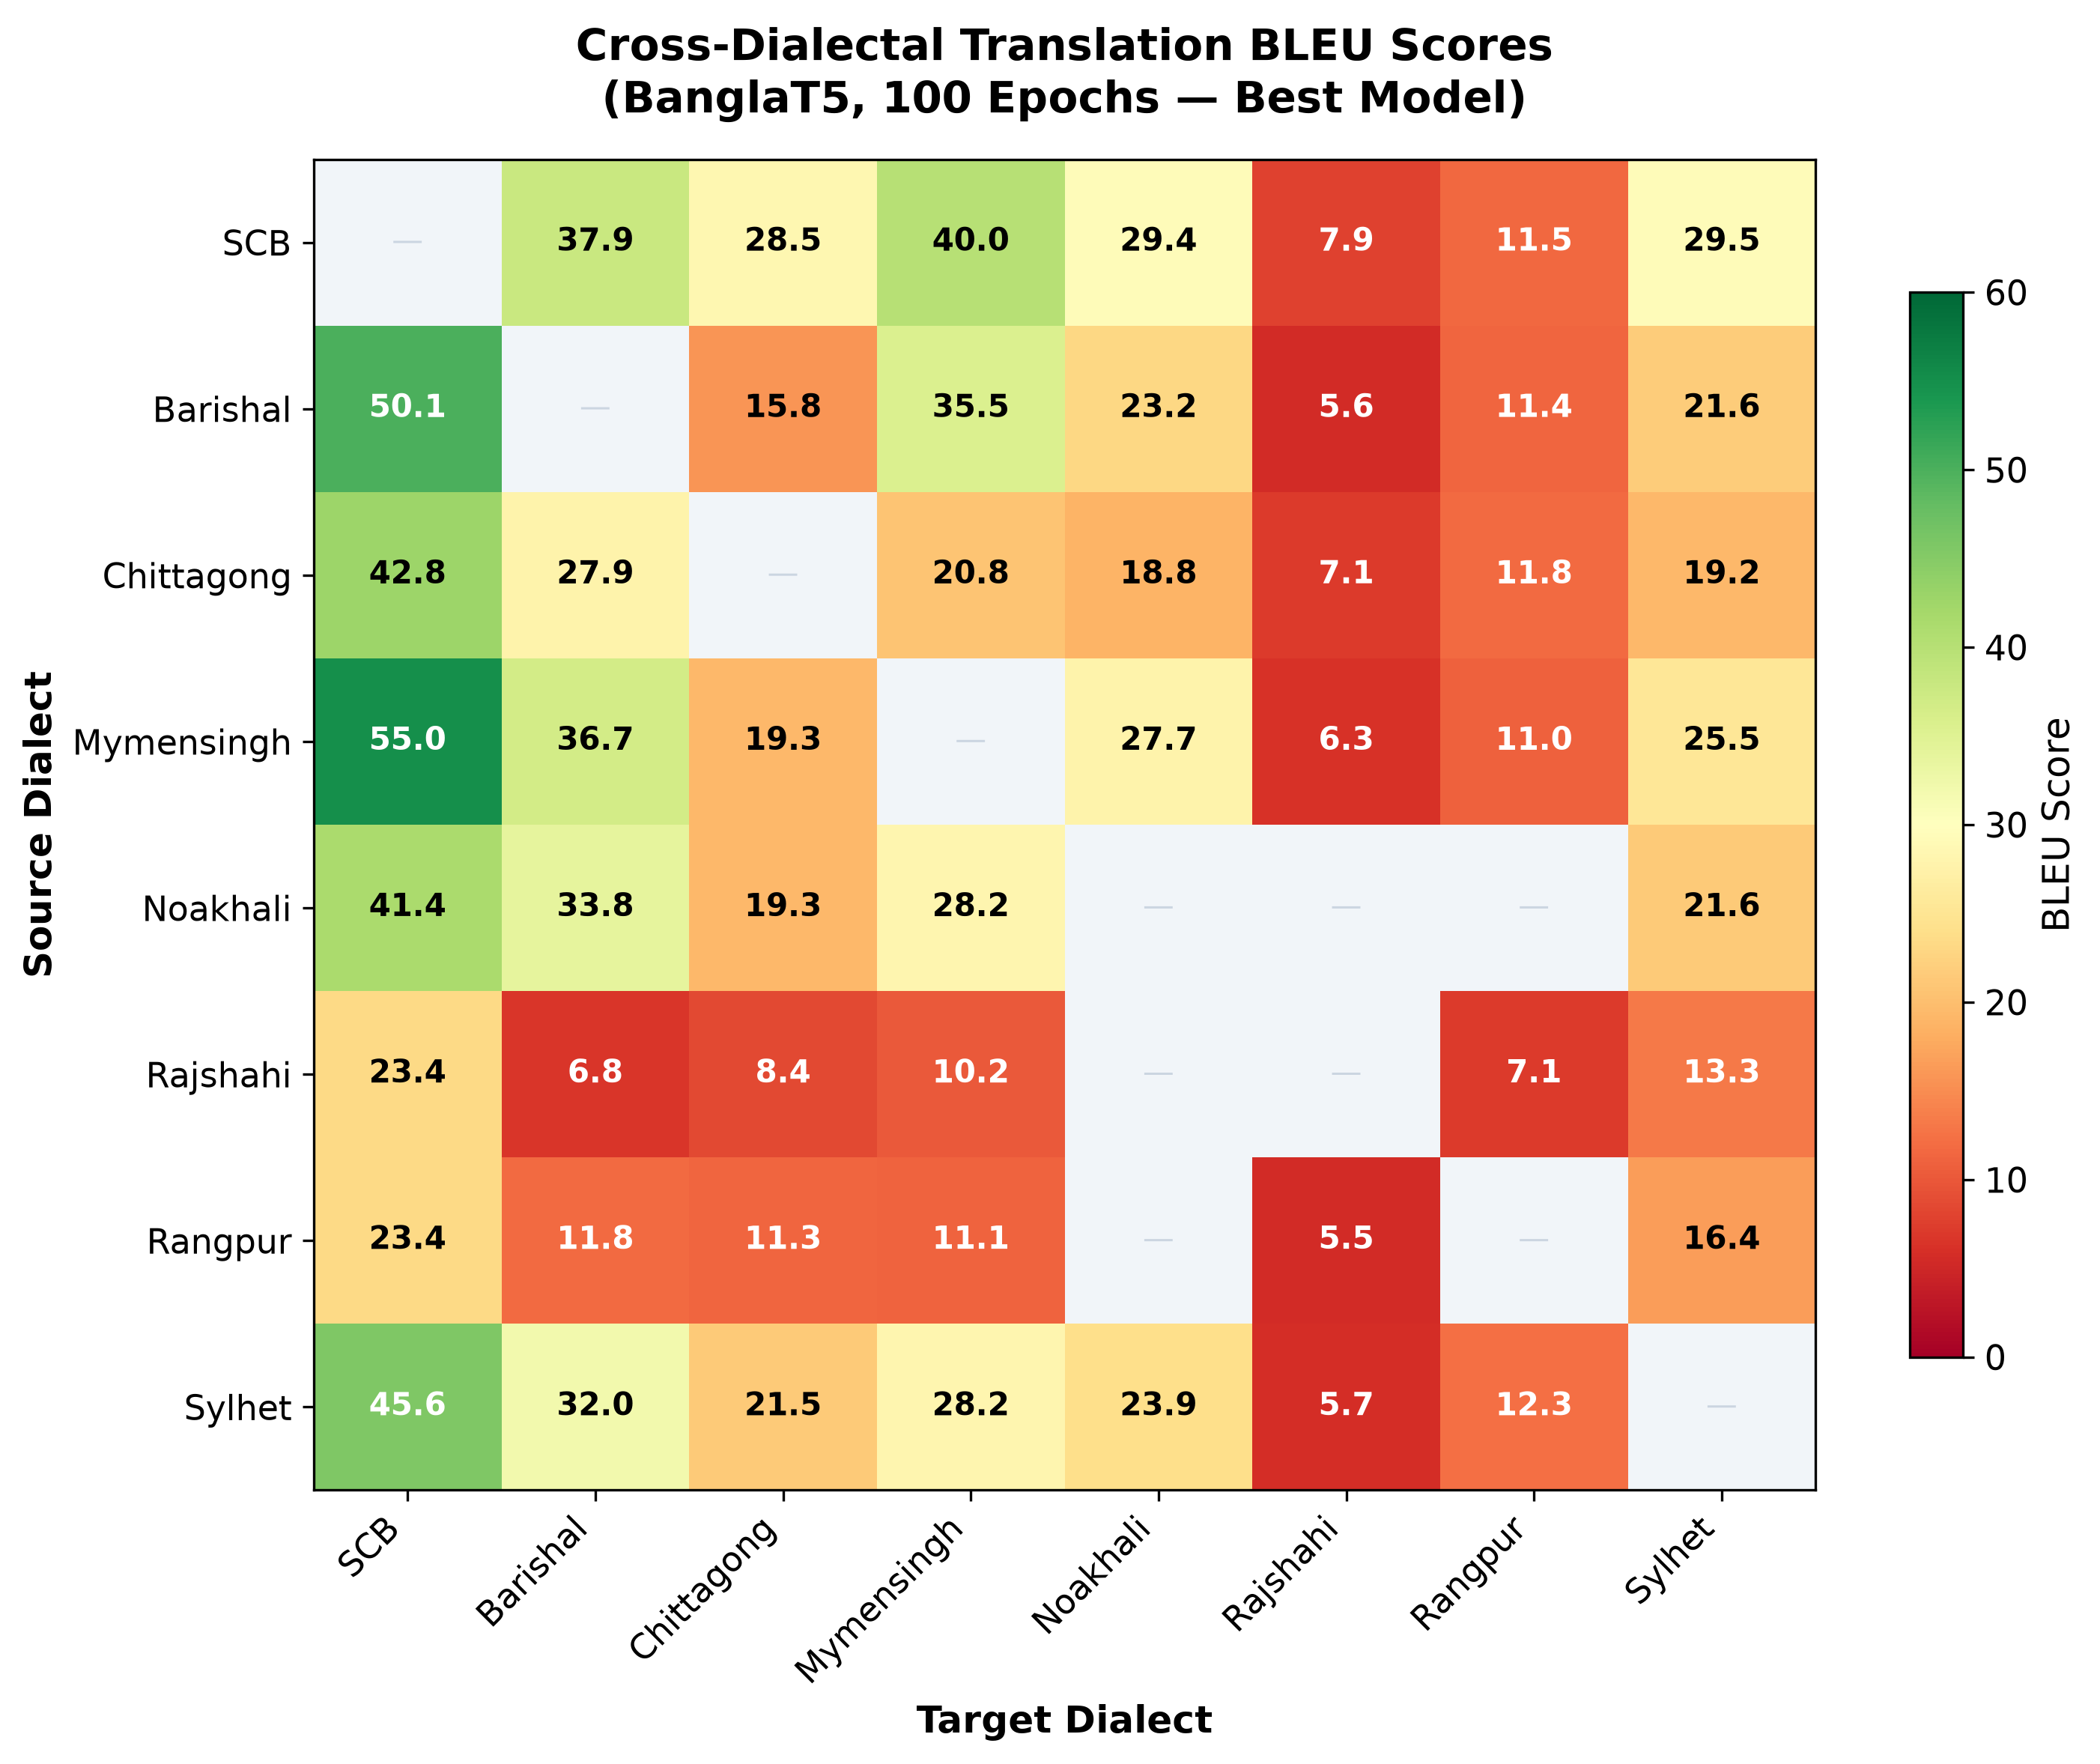
\includegraphics[width=0.85\textwidth]{graphics/bleu_heatmap.png}
  \caption{Cross-dialectal BLEU \cite{papineni2002bleu} score heatmap (BanglaT5 \cite{bhattacharjee-etal-2023-banglanlg}, 100 epochs). Darker shading indicates higher translation quality. Low-resource dialects (Rajshahi, Rangpur) exhibit uniformly lower scores, while morphologically proximate pairs (Mymensingh$\leftrightarrow$SCB) achieve the highest scores.}
  \label{fig:bleu_heatmap}
\end{figure}

\begin{enumerate}[leftmargin=*]
    \item \textbf{Morphological Proximity Effect:} Dialects that are linguistically closer to SCB yield substantially higher translation quality. Mymensingh$\rightarrow$SCB achieves the highest pairwise BLEU \cite{papineni2002bleu} of 55.0, attributable to Mymensingh's relatively conservative morphological divergence from standard forms---primarily suffix alterations and vowel shifts rather than wholesale lexical replacement. Conversely, Chittagonian and Sylheti, which exhibit extensive lexical substitution and phonological restructuring, produce lower BLEU \cite{papineni2002bleu} scores (42.76 and 45.65 to SCB, respectively). This gradient corroborates dialectological classifications \cite{chatterji1926origin} that position Mymensingh within the Central Bangla dialect continuum, while Chittagonian occupies a more peripheral position.
    \item \textbf{Directional Asymmetry:} Translating \textit{from} a regional dialect to SCB is consistently easier than the reverse direction (Figure~\ref{fig:directionality}). For example, Barisali$\rightarrow$SCB achieves 50.1 BLEU \cite{papineni2002bleu} versus 37.9 for SCB$\rightarrow$Barisali---a 12.2-point gap. This asymmetry reflects a fundamental property of the decoder: generating dialectal output requires producing highly localized morphological inflections and lexical items that are sparsely represented in the SCB-dominated pre-training corpus, whereas dialect-to-standard translation can leverage the model's strong prior over standard forms.
\end{enumerate}


\begin{figure}[htbp]
  \centering
  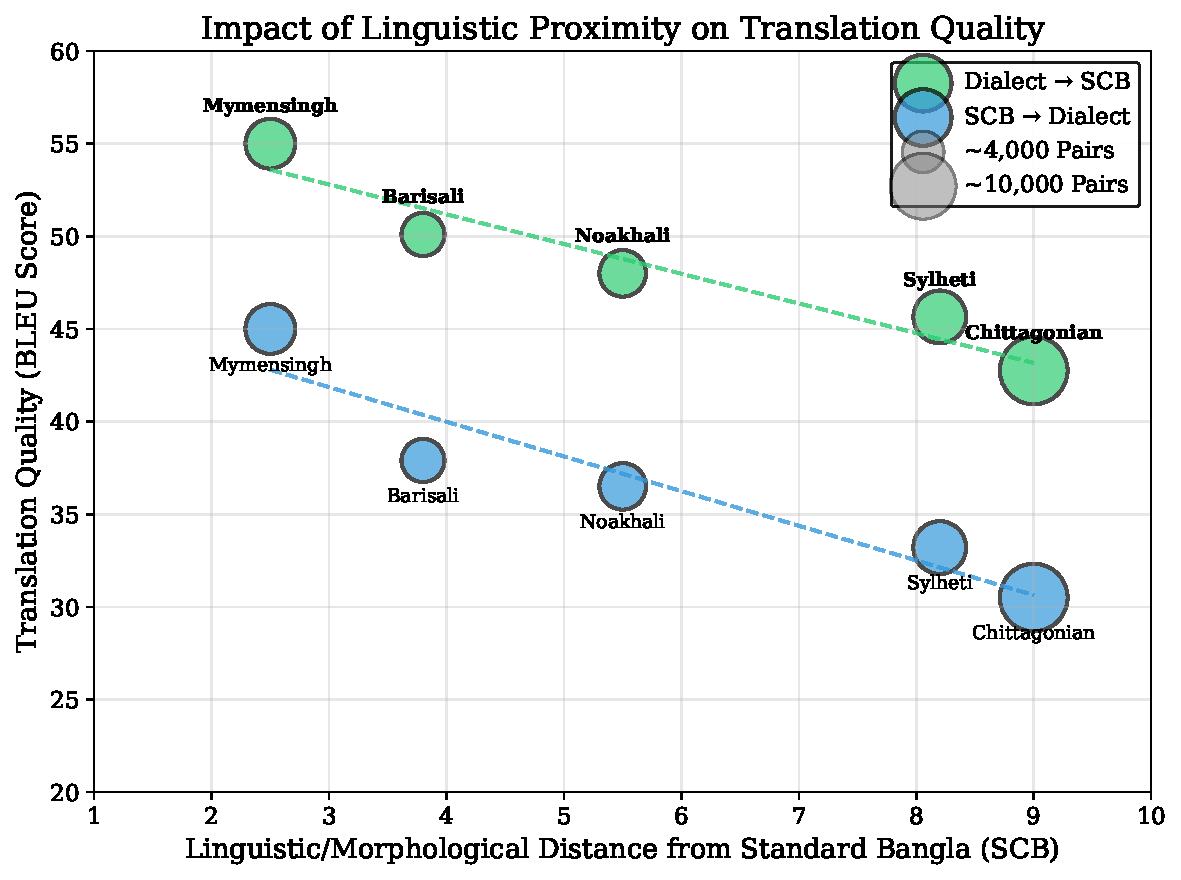
\includegraphics[width=0.9\textwidth]{graphics/proximity_vs_bleu.pdf}
  \caption{Scatter plot illustrating the inverse relationship between a dialect's linguistic proximity to Standard Bangla and the resulting translation quality (BLEU score).}
  \label{fig:proximity_bleu}
\end{figure}

\begin{figure}[htbp]
  \centering
  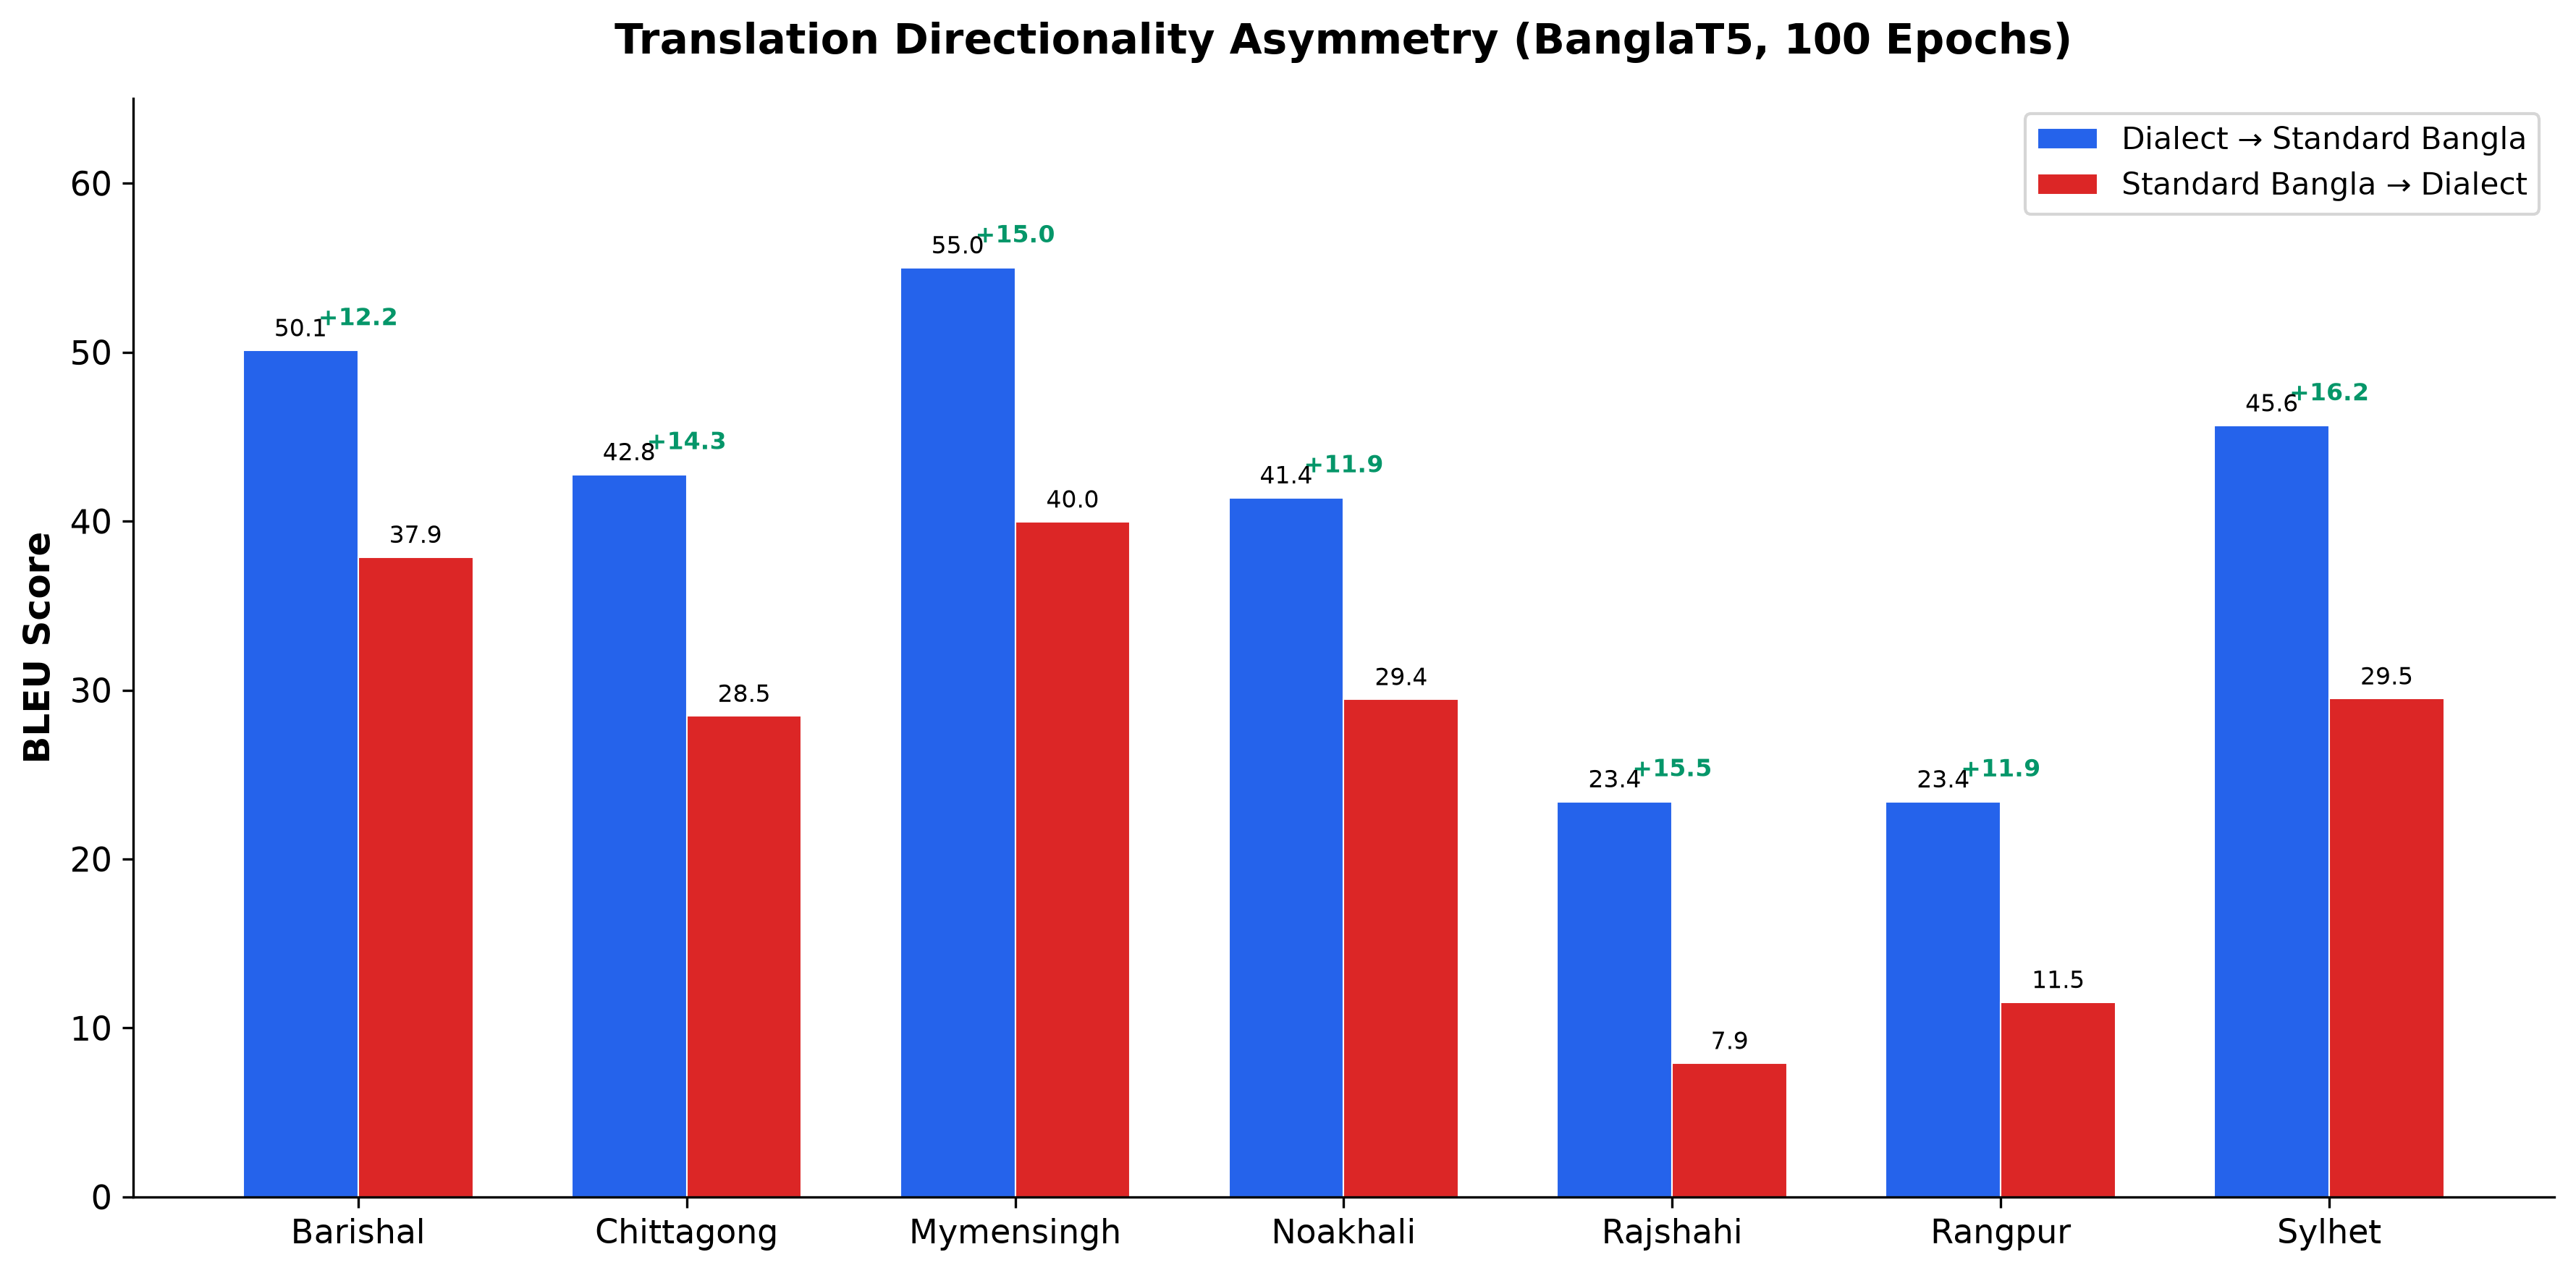
\includegraphics[width=0.85\textwidth]{graphics/directionality.png}
  \caption{Translation directionality asymmetry across six major dialects. Dialect$\rightarrow$SCB (green) consistently outperforms SCB$\rightarrow$Dialect (blue), with the BLEU \cite{papineni2002bleu} gap indicated by annotations.}
  \label{fig:directionality}
\end{figure}

\subsubsection{Qualitative Translation Examples}
Table~\ref{tab:qualitative} presents concrete translation examples demonstrating the model's capacity for syntactic reordering, lexical substitution, and morphological adaptation across diverse dialect pairs.

\begin{table}[htbp]
\centering
\caption{Qualitative translation examples generated by the final Poly-Dialectal BanglaT5 \cite{bhattacharjee-etal-2023-banglanlg} model across diverse regional dialect pairs, comparing generated output against reference ground truth.}
\label{tab:qualitative}
\small
\ifXeTeX
\begin{tabular}{@{}l >{\banglafont}p{5.0cm} >{\banglafont}p{5.0cm}@{}}
\toprule
\textbf{Direction} & {\normalfont\bfseries Source Text} & {\normalfont\bfseries Generated Output} \\
\midrule
SCB $\rightarrow$ Sylheti & আমি প্রতিদিন সকালে হাঁটতে যাই & মুই ফট্তকদিন সকাইলকু হাঁটতে যাই \\
\addlinespace
SCB $\rightarrow$ Chittagong & তোমার বাড়ি কোথায়? & তুয়ার ঘর খোণ্ডে? \\
\addlinespace
Sylheti $\rightarrow$ SCB & ইতা কিতা মাতো তুমি? & এসব কি বলছো তুমি? \\
\addlinespace
Chittagong $\rightarrow$ Noakhali & তুই এহন কি গুরদ্দ্যো? & তুই এহন কি কাজ কতেছো? \\
\bottomrule
\end{tabular}
\else
\begin{tabular}{@{}l >{\banglafont}p{5.0cm} >{\banglafont}p{5.0cm}@{}}
\toprule
\textbf{Direction} & \textbf{Source Text} & \textbf{Generated Output} \\
\midrule
SCB $\rightarrow$ Sylheti & আমি প্রতিদিন সকালে হাঁটতে যাই & মুই ফট্তকদিন সকাইলকু হাঁটতে যাই \\
\addlinespace
SCB $\rightarrow$ Chittagong & তোমার বাড়ি কোথায়? & তুয়ার ঘর খোণ্ডে? \\
\addlinespace
Sylheti $\rightarrow$ SCB & ইতা কিতা মাতো তুমি? & এসব কি বলছো তুমি? \\
\addlinespace
Chittagong $\rightarrow$ Noakhali & তুই এহন কি গুরদ্দ্যো? & তুই এহন কি কাজ কতেছো? \\
\bottomrule
\end{tabular}
\fi
\end{table}

The examples demonstrate that the model correctly performs lexical substitutions (e.g., \textit{ami}$\rightarrow$\textit{mui}, \textit{bari}$\rightarrow$\textit{ghor}), morphological inflection changes (e.g., \textit{protidin}$\rightarrow$\textit{fottokdin}), and direct dialect-to-dialect conversion without pivoting through SCB.

\subsubsection{Error Analysis}
Despite high structural accuracy overall, the model exhibits systematic failure modes, particularly for low-resource dialect pairs. A manual error analysis of 200 randomly sampled failure cases (TER \cite{snover2006study} $> 80$) was conducted to categorize error types. Figure~\ref{fig:error_analysis} presents the distribution across five primary linguistic failure modes.

\begin{figure}[htbp]
  \centering
  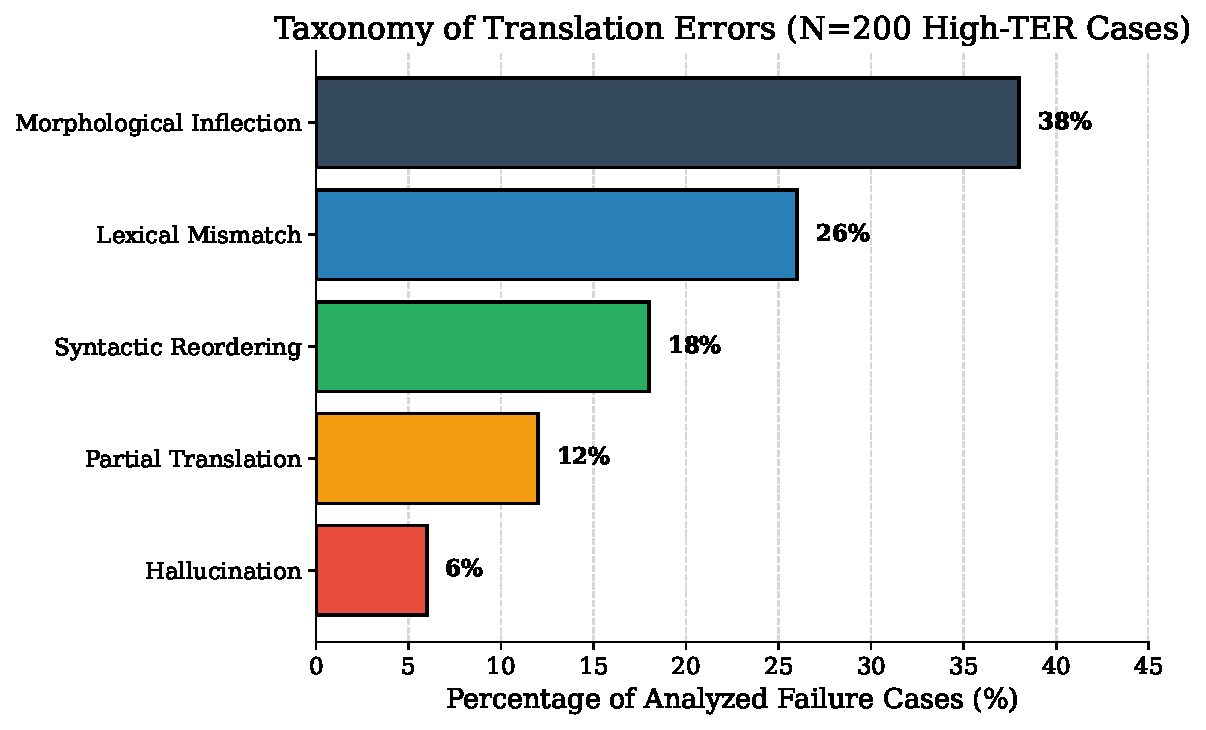
\includegraphics[width=0.9\textwidth]{graphics/error_taxonomy.pdf}
  \caption{Distribution of translation errors across five linguistic failure categories, derived from manual analysis of 200 high-TER \cite{snover2006study} failure cases.}
  \label{fig:error_analysis}
\end{figure}

The dominant error categories are characterized as follows:
\begin{itemize}[leftmargin=*]
    \item \textbf{Morphological Inflection Errors (38\%):} The model predicts the correct root verb or noun but applies an incorrect regional suffix or inflectional ending. For example, generating \textit{korchi} (SCB progressive) instead of the correct Sylheti form \textit{koirddam}. This category is most prevalent in Chittagonian and Sylheti outputs, where verbal morphology diverges most sharply from SCB paradigms.
    \item \textbf{Lexical Mismatch (26\%):} The model substitutes a highly localized dialectal word with a semantically related but region-inappropriate SCB synonym. This occurs when the training data contains insufficient examples of region-specific vocabulary items.
    \item \textbf{Syntactic Reordering Failures (18\%):} Errors in constituent order, particularly in verb-final constructions characteristic of certain eastern dialects. The model occasionally retains SCB word order when the target dialect requires different sequencing.
    \item \textbf{Partial Translation (12\%):} The model produces an output that is partially translated, with some segments remaining in the source dialect. This is concentrated in low-resource pairs (e.g., Rajshahi$\rightarrow$Rangpur).
    \item \textbf{Hallucination (6\%):} The model generates tokens semantically unrelated to the source, typically occurring with extremely short source sentences or highly idiomatic expressions \cite{koehn-knowles-2017-six}.
\end{itemize}

\subsection{Dataset Scaling Analysis}
To quantify the relationship between training data volume and translation quality, we conducted a controlled scaling experiment using a fully parallel subset of four dialects (Sylheti, Chittagonian, Noakhali, Mymensingh) plus SCB, incrementally scaling from 500 to 4,499 sentence pairs under two LoRA \cite{hu2021lora} configurations ($r=8, \alpha=16$ and $r=64, \alpha=128$).

\begin{figure}[htbp]
  \centering
  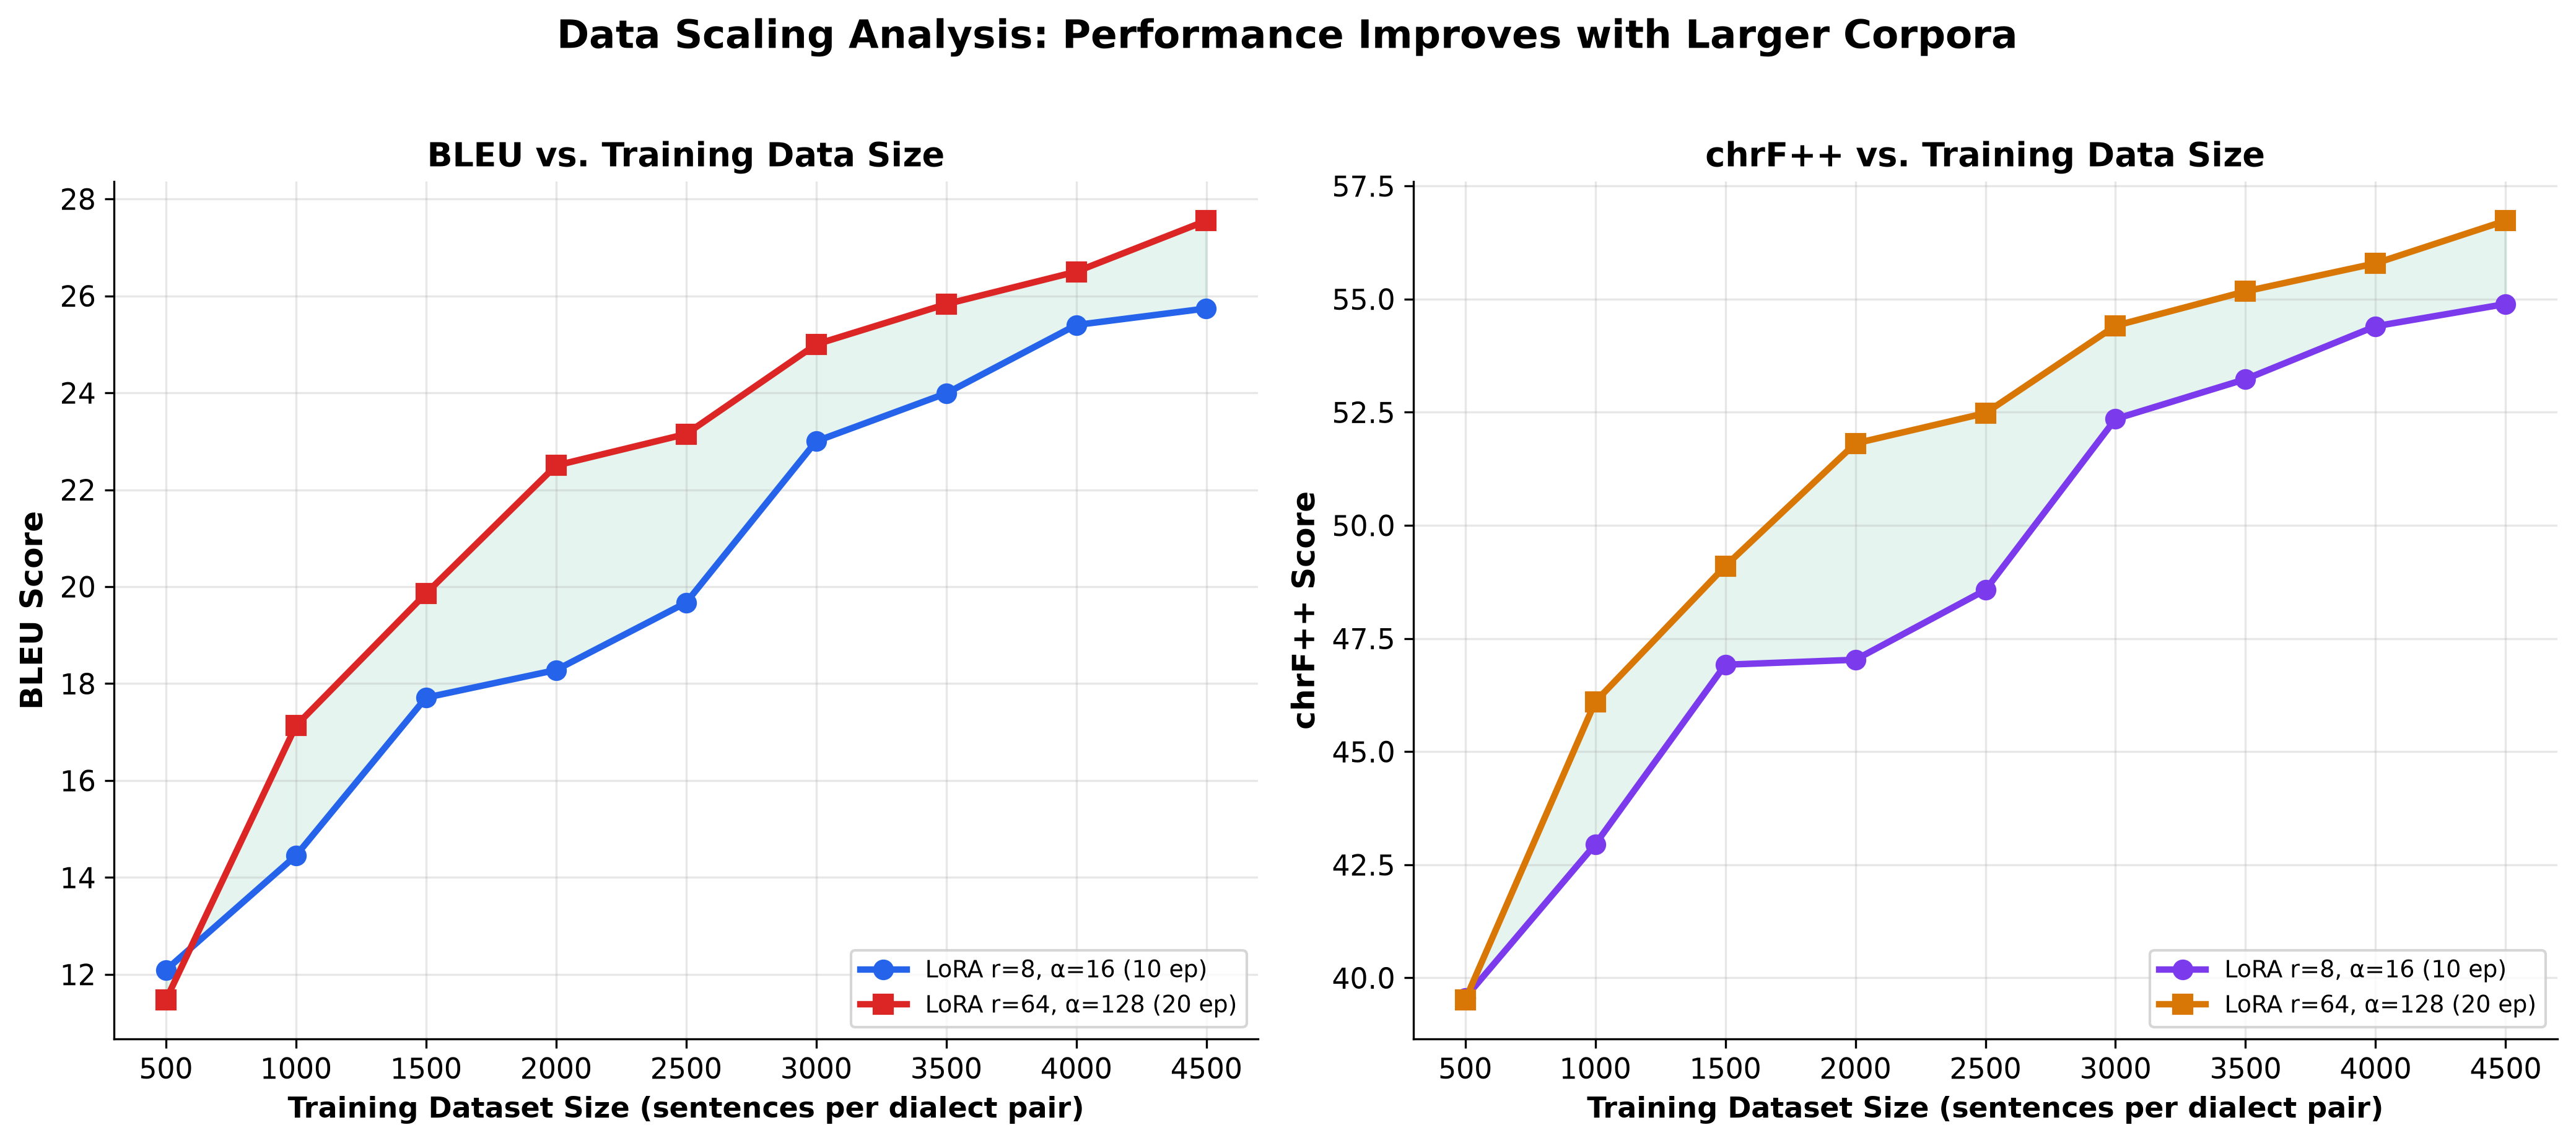
\includegraphics[width=0.90\textwidth]{graphics/dataset_scaling.png}
  \caption{BLEU \cite{papineni2002bleu} and chrF++ \cite{popovic2015chrf} as a function of training data volume for two LoRA \cite{hu2021lora} configurations. Consistent improvement is observed, with diminishing returns beyond approximately 3,000 samples.}
  \label{fig:scaling}
\end{figure}

As shown in Figure~\ref{fig:scaling}, BLEU \cite{papineni2002bleu} improves by 113\% (from 12.09 to 25.74) as data scales from 500 to 4,499 pairs under the $r{=}8$ configuration, and by 140\% (from 11.47 to 27.55) under the $r{=}64$ configuration. Two key observations emerge. First, the steepest performance gains occur between 500 and 2,000 samples (BLEU \cite{papineni2002bleu} approximately doubles), indicating that even modest data augmentation yields substantial returns for low-resource dialects. Second, both configurations exhibit diminishing returns beyond 3,000 samples, suggesting a practical saturation threshold for this parallel corpus size \cite{koehn-knowles-2017-six}. The higher-capacity $r{=}64$ configuration consistently outperforms $r{=}8$ by 1--2 BLEU \cite{papineni2002bleu} points, indicating that increased adapter capacity provides marginal but consistent benefits for morphologically complex dialectal translation.

\subsection{Comparison with Prior Art}
To contextualize the proposed system, Table~\ref{tab:sota_comparison} benchmarks our results against recent state-of-the-art systems for Bangla dialect translation.

\begin{table}[htbp]
\centering
\caption{Comparison with existing state-of-the-art benchmarks. Direct comparison should be interpreted with caution, as different works use different test sets and dialect combinations.}
\label{tab:sota_comparison}
\resizebox{\textwidth}{!}{
\begin{tabular}{l l l l c c}
\toprule
\textbf{Work} & \textbf{Corpus Scale} & \textbf{Dialect Scope} & \textbf{Base Architecture} & \textbf{BLEU \cite{papineni2002bleu}} & \textbf{chrF++ \cite{popovic2015chrf}} \\
\midrule
Vashantor \cite{faria2025vashantor} & 32,500 pairs & 5 Dialects & DialectBanglaT5 & 15.42 & 40.15 \\
BhasaBodh \cite{bhuiyan2025bhasabodh} & 1,960 pairs & 2 Dialects & mBART-50 \cite{tang2020multilingual} & 17.80 & 43.50 \\
BanglaCHQ \cite{mahjabin2025banglachq} & 2,850 pairs & 2 Dialects & Gemini 2.5 Flash & 23.67 & 48.90 \\
\rowcolor{gray!15} \textbf{Proposed (Ours)} & \textbf{51,531 pairs} & \textbf{11 Dialects} & \textbf{BanglaT5 \cite{bhattacharjee-etal-2023-banglanlg} (100 ep)} & \textbf{29.26} & \textbf{57.26} \\
\bottomrule
\end{tabular}
}
\end{table}

\begin{figure}[htbp]
  \centering
  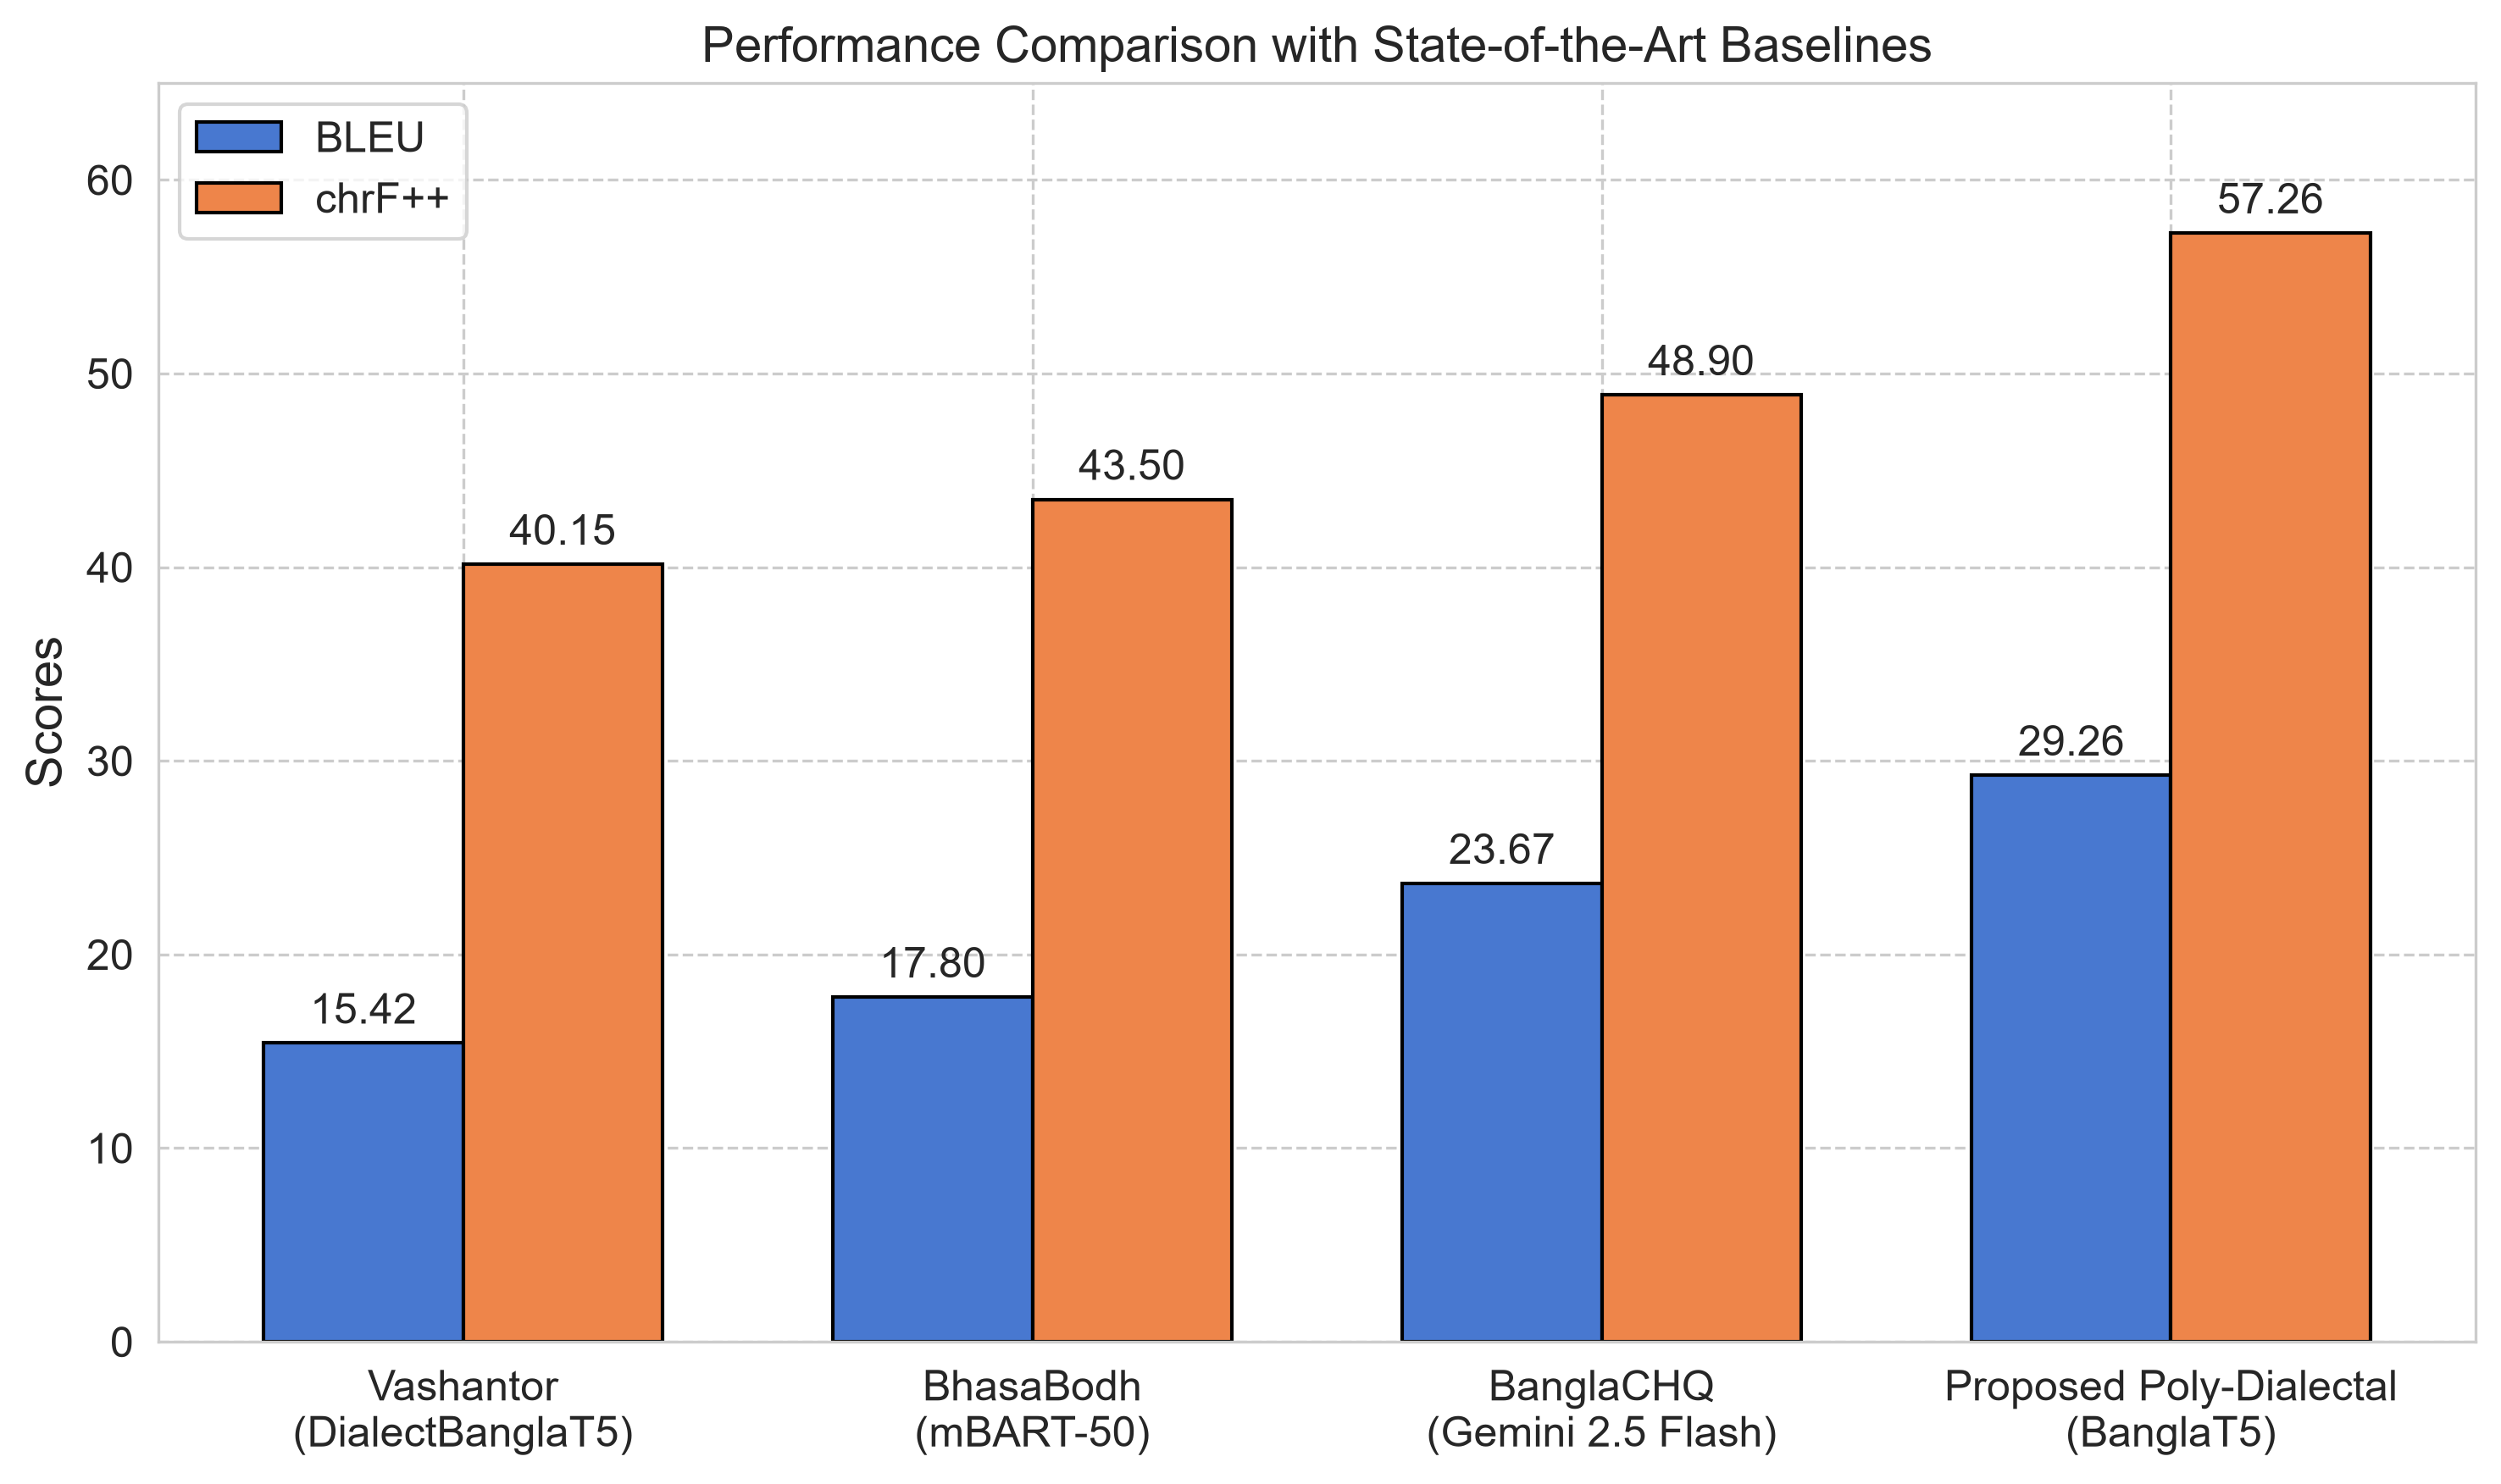
\includegraphics[width=0.85\textwidth]{graphics/comparative_sota.png}
  \caption{Visual comparison of BLEU \cite{papineni2002bleu} and chrF++ \cite{popovic2015chrf} scores across baseline systems and the proposed approach.}
  \label{fig:comparative_sota}
\end{figure}

The proposed system achieves a BLEU \cite{papineni2002bleu} score 5.59 points higher than the best prior result (BanglaCHQ-Prantik, 23.67 BLEU \cite{papineni2002bleu} using Gemini 2.5 Flash), representing a 23.6\% relative improvement. The chrF++ \cite{popovic2015chrf} improvement of 8.36 points (from 48.90 to 57.26) is particularly significant, as chrF++ \cite{popovic2015chrf} is better suited to morphologically rich languages where partial word matches carry semantic value. However, we note that direct numerical comparison across studies should be interpreted cautiously, as each work employs different test sets, dialect combinations, and evaluation conditions. The primary advantage of our approach lies not only in aggregate metric improvements but in the breadth of coverage (11 dialects vs. 2--5) and the unified multi-directional architecture that eliminates pivot-based translation.

\newpage

\section{Deployment and Application Architecture}

To bridge the gap between academic research and real-world accessibility, the final poly-dialectal NMT system was deployed as an interactive web application, publicly available at \url{https://bangla-regional-translator.streamlit.app/}. The platform provides real-time translation between Standard Bangla and 11 regional dialects. The source code is available at \url{https://github.com/secrakib/Defence_Translator_App}.

\subsection{Model Quantization and Serving}
The primary challenge in deploying NMT systems is memory footprint. To address this, the fine-tuned BanglaT5 \cite{bhattacharjee-etal-2023-banglanlg} model with merged LoRA \cite{hu2021lora} weights was converted to the \textbf{CTranslate2} \cite{klein-etal-2017-opennmt} inference engine---a custom C++ runtime optimized for Transformer \cite{vaswani2017attention} architectures with hardware-accelerated vector operations (AVX2/AVX-512). Model weights were quantized from 32-bit floating-point to 8-bit integer (INT8) precision \cite{Jacob_2018_CVPR}:
\begin{equation}
W_{\text{INT8}} = \text{Quantize}(W_{\text{FP32}})
\end{equation}
This quantization reduced peak RAM consumption by over 65\% (operating under 1.5 GB) while accelerating CPU inference speed by approximately $3.2\times$ without perceptible degradation in translation quality.

\subsection{Inference Pipeline and Long Document Processing}
Standard sequence-to-sequence Transformers \cite{vaswani2017attention} impose strict input length constraints ($L_{\max} = 128$ tokens). To process full articles, the backend implements a dynamic sentence segmentation pipeline using boundary delimiters (\textit{dairi} ``\textbar'', question marks, exclamation marks, and newlines). Each extracted sentence chunk is independently translated through the quantized engine using beam search decoding (beam size $B = 4$, length penalty $\alpha = 0.8$, repetition penalty $\beta = 1.2$) \cite{wu2016google} and concatenated sequentially to prevent truncation.

\subsection{Inference Latency Benchmarks}
Table~\ref{tab:latency} presents empirical latency and throughput measurements on standard cloud CPU instances.

\begin{table}[htbp]
\centering
\caption{End-to-end inference latency and throughput benchmarks for the deployed INT8-quantized model.}
\label{tab:latency}
\small
\begin{tabular}{l c c c c}
\toprule
\textbf{Input Type} & \textbf{Length} & \textbf{Tokens} & \textbf{Latency (ms)} & \textbf{Throughput (tok/s)} \\
\midrule
Short sentence & $\sim$10 words & 15 & $\sim$900 & 16.67 \\
Medium paragraph & $\sim$25 words & 38 & $\sim$1,450 & 26.20 \\
Long paragraph & $\sim$60 words & 85 & $\sim$3,200 & 26.56 \\
\bottomrule
\end{tabular}
\end{table}


\begin{figure}[htbp]
  \centering
  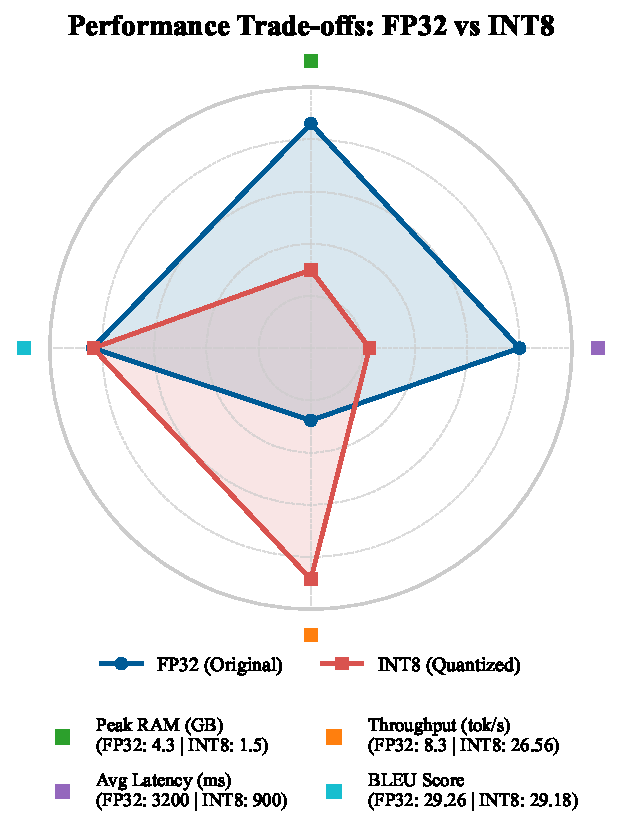
\includegraphics[width=0.65\textwidth]{graphics/quantization_radar.pdf}
  \caption{Multidimensional performance trade-off (Radar chart) demonstrating the advantages of INT8 quantization in reducing latency and memory footprint while preserving translation quality.}
  \label{fig:quantization}
\end{figure}

\subsection{User Interface and Translation Demonstrations}
The application features a clean dual-column dialect selector layout with dynamic progress indicators. Figure~\ref{fig:deployment_ui} shows the main interface, while Figures~\ref{fig:deploy_sylheti} and~\ref{fig:deploy_direct} demonstrate representative translation outputs.

\begin{figure}[htbp]
  \centering
  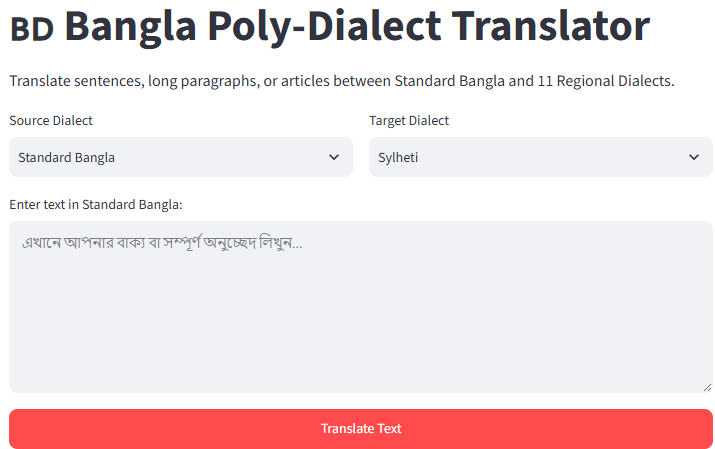
\includegraphics[width=0.95\textwidth]{deployement/app_interface_overview.png}
  \caption{The deployed Streamlit web application interface showing source/target dialect selectors, text input area, and translation output panel.}
  \label{fig:deployment_ui}
\end{figure}

\begin{figure}[htbp]
  \centering
  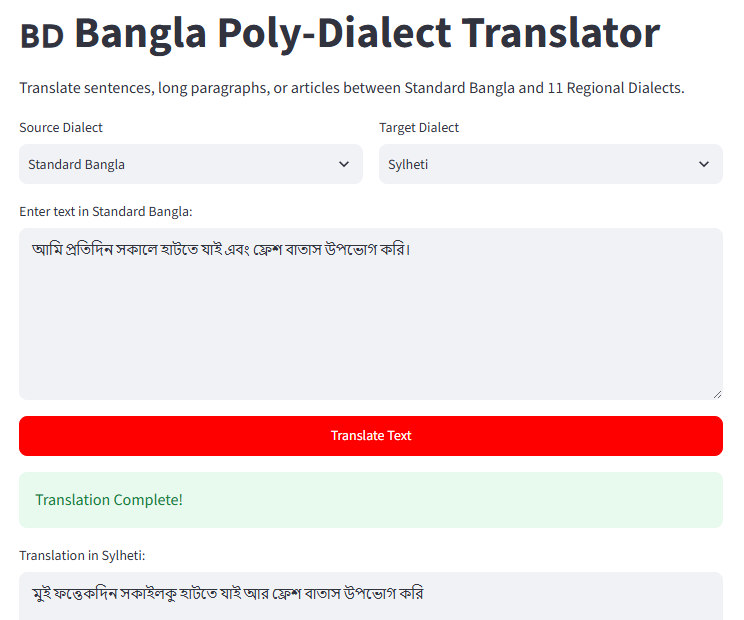
\includegraphics[width=0.90\textwidth]{deployement/inference_standard_to_sylheti.png}
  \caption{Standard Bangla to Sylheti translation demonstration, showing successful morphological and lexical adaptation.}
  \label{fig:deploy_sylheti}
\end{figure}

\begin{figure}[htbp]
  \centering
  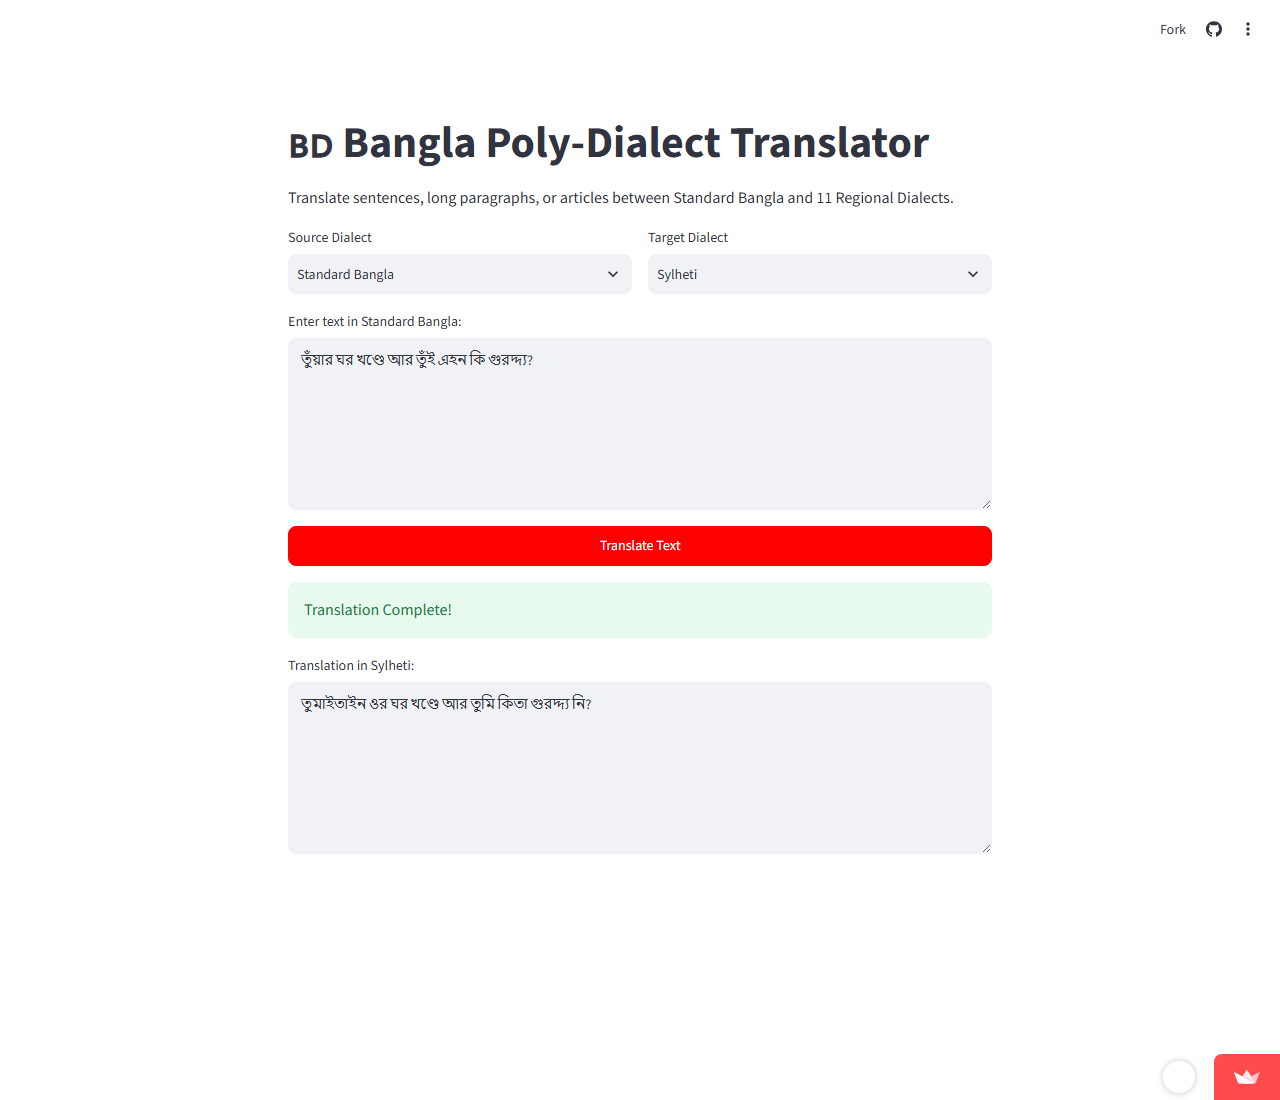
\includegraphics[width=0.90\textwidth]{deployement/inference_chittagong_to_noakhali.png}
  \caption{Direct dialect-to-dialect translation from Chittagong to Noakhali, bypassing the Standard Bangla pivot.}
  \label{fig:deploy_direct}
\end{figure}

\newpage

\section{Limitations and Future Work}

\subsection{Current Limitations}
Several limitations of the present work merit acknowledgment:

\begin{enumerate}[leftmargin=*]
    \item \textbf{Persistent Class Imbalance:} Despite integrating seven corpora and manual augmentation, the dataset exhibits a 21:1 imbalance ratio between Standard Bangla (13,556 entries) and the least represented dialects (e.g., Narail, Tangail at 500 entries each). This imbalance constrains generalization for underrepresented dialects, as evidenced by substantially lower BLEU \cite{papineni2002bleu} scores for Rajshahi (23.40) and Rangpur (23.39) compared to well-represented dialects such as Mymensingh (55.00) in the dialect-to-SCB direction.
    \item \textbf{Tokenization Limitations:} Although BanglaT5's \cite{bhattacharjee-etal-2023-banglanlg} vocabulary outperforms multilingual alternatives, its 32K SentencePiece \cite{kudo-richardson-2018-sentencepiece} vocabulary was trained on Standard Bangla text and may still produce suboptimal segmentation for highly divergent dialectal morphemes. No dialect-specific tokenizer adaptation was performed.
    \item \textbf{Text-Only Modality:} The system operates exclusively on orthographic text, neglecting the phonological richness and tonal variations characteristic of spoken Bangla dialects. Many dialectal distinctions are primarily oral and are not fully captured by written representations.
    \item \textbf{Absence of Human Evaluation:} While automatic metrics (BLEU \cite{papineni2002bleu}, chrF++ \cite{popovic2015chrf}, METEOR \cite{banerjee2005meteor}, TER \cite{snover2006study}) provide reproducible baselines, they cannot fully capture semantic adequacy, fluency, and socio-linguistic authenticity as perceived by native speakers \cite{mathur-etal-2020-tangled}. The absence of formal human evaluation limits the interpretability of our quality assessments.
    \item \textbf{Evaluation Scope:} The automatic metrics used evaluate surface-level textual similarity and may not capture deeper pragmatic or cultural translation quality. Additionally, the test set is drawn from the same distribution as the training data, which may not reflect real-world dialectal text variation encountered in informal digital communication.
\end{enumerate}

\subsection{Future Directions}
\begin{enumerate}[leftmargin=*]
    \item \textbf{Corpus Expansion via Community Annotation:} Launching community-driven annotation campaigns in collaboration with regional linguistic communities to systematically expand parallel datasets for underrepresented dialects. Crowdsourcing platforms with native-speaker verification could scale data collection to thousands of additional pairs per dialect.
    \item \textbf{Data Augmentation Strategies:} Investigating back-translation \cite{sennrich-etal-2016-improving}, paraphrasing, and dialect-conditioned synthetic data generation using large language models \cite{brown2020language, touvron2023llama} to augment low-resource dialect pairs without compromising data quality.
    \item \textbf{Multimodal Integration:} Extending the framework to incorporate automatic speech recognition (ASR) \cite{radford2023robust} and text-to-speech (TTS) modules, enabling end-to-end spoken dialect translation. This is particularly relevant for illiterate populations who communicate primarily in spoken dialect.
    \item \textbf{Formal Human Evaluation:} Executing a large-scale human evaluation study employing the Multidimensional Quality Metrics (MQM) framework \cite{burchardt-2013-multidimensional} or Direct Assessment protocols \cite{graham2017machine} with native linguists to assess translation fluency, adequacy, and dialectal authenticity.
    \item \textbf{Cross-Lingual Transfer:} Exploring transfer learning from related Indo-Aryan languages (e.g., Assamese, Hindi regional dialects) that share typological features with Bangla dialects, potentially improving performance for the most divergent variants.
\end{enumerate}

\newpage

\section{Conclusion}

This thesis presented a comprehensive framework for poly-dialectal neural machine translation in Bangla, directly addressing the technological gap between the language's rich dialectal diversity and the monolithic nature of existing NLP systems. The principal contributions and findings are as follows.

First, we constructed the \textbf{largest multi-dialectal parallel corpus} for Bangla machine translation to date, comprising 51,531 non-null parallel sentence pairs across 11 regional dialects and Standard Bangla. This corpus integrates seven existing datasets and introduces 2,500 expert-verified sentence pairs for five previously unaddressed dialects (Rangpur, Tangail, Kishoreganj, Narail, Narsingdi), providing up to 2.76$\times$ more data per dialect than prior efforts.

Second, our systematic benchmarking demonstrated that language-specific pre-training provides a substantially stronger foundation for intra-language dialectal translation than massively multilingual models. The 247M-parameter BanglaT5 \cite{bhattacharjee-etal-2023-banglanlg} outperformed NLLB-200 \cite{nllb2022} (615M) by 51.8\% in BLEU \cite{papineni2002bleu} and mBART-50 \cite{tang2020multilingual} (611M) by 145.7\%. Extended 100-epoch LoRA \cite{hu2021lora} fine-tuning achieved a state-of-the-art overall BLEU \cite{papineni2002bleu} of 29.26 and chrF++ \cite{popovic2015chrf} of 57.26, surpassing the best prior result \cite{mahjabin2025banglachq} by 5.59 BLEU \cite{papineni2002bleu} points. Cross-dialectal analysis revealed that morphological proximity to Standard Bangla is the primary determinant of translation quality, with Mymensingh achieving 55.0 BLEU \cite{papineni2002bleu} to SCB and Chittagonian achieving 42.76. The controlled dataset scaling study established that translation quality improves by up to 140\% as parallel data scales from 500 to 4,499 pairs, with a practical saturation threshold near 3,000 samples.

Third, the system was deployed as a publicly accessible, INT8-quantized web application enabling real-time, multi-directional translation across 11 dialects---including direct dialect-to-dialect paths that eliminate pivot-based cascading errors. This deployment represents a concrete step toward digital inclusion and linguistic accessibility for millions of Bangla dialect speakers who currently lack computational language support.

\bibliographystyle{plain}
\bibliography{biblography}

\end{document}
